\documentclass[11pt,a4paper]{article}
\usepackage[utf8]{inputenc}
\usepackage[english]{babel}
\usepackage{graphicx}
\usepackage{amssymb}				% Símbolos de números
\usepackage[hidelinks]{hyperref}	% Con hidelinks no se muestran los recuadros rojos
\usepackage{tikz}
\usetikzlibrary{automata, positioning, arrows, trees}

% Ajustar tikzet
\tikzset{
	->, % Hace que los arcos sean dirigidos
	>=stealth, % Hace que la punta de las flechas sean gruesas
	node distance=3cm, % Distancia minima entre nodos
	every state/.style={thick}, % Propiedades de los nodos
	initial text=$ $ % Texto que aparece en el estado inicial
}

\usepackage{makecell}
\usepackage{float}
\usepackage[shortlabels]{enumitem}	% Para enumeraciones con letras
\usepackage[textwidth=390pt]{geometry}


%Códigos fuente
\usepackage{listings}
\usepackage{color}
\usepackage{graphicx}

\definecolor{mygreen}{rgb}{0,0.6,0}
\definecolor{mygray}{rgb}{0.5,0.5,0.5}
\definecolor{mymauve}{rgb}{0.58,0,0.82}

\lstset{ 
  backgroundcolor=\color{white},   % choose the background color
  basicstyle=\footnotesize,        % the size of the fonts that are used for the code
  breakatwhitespace=false,         % sets if automatic breaks should only happen at whitespace
  breaklines=true,                 % sets automatic line breaking
  captionpos=b,                    % sets the caption-position to bottom
  commentstyle=\color{mygreen},    % comment style
  deletekeywords={...},            % if you want to delete keywords from the given language
  escapeinside={\%*}{*)},          % if you want to add LaTeX within your code
  extendedchars=true,              % lets you use non-ASCII characters; for 8-bits encodings only, does not work with UTF-8
  frame=single,                    % adds a frame around the code
  keepspaces=true,                 % keeps spaces in text, useful for keeping indentation of code (possibly needs columns=flexible)
  keywordstyle=\color{blue},       % keyword style
  language=C,                     % the language of the code
  morekeywords={*,private},        % add more keywords to the set
  numbers=left,                    % where to put the line-numbers (none, left, right)
  numbersep=5pt,                   % how far the line-numbers are from the code
  numberstyle=\tiny\color{mygray}, % the style that is used for the line-numbers
  rulecolor=\color{black},         % if not set, the frame-color may be changed on line-breaks within not-black text
  showspaces=false,                % show spaces everywhere adding particular underscores; it overrides 'showstringspaces'
  showstringspaces=false,          % underline spaces within strings only
  showtabs=false,                  % show tabs within strings adding particular underscores
  stepnumber=1,                    % the step between two line-numbers. If 1, each line si numbered
  stringstyle=\color{magenta},     % string literal style
  tabsize=2,                    % sets default tabsize to 2 spaces
  title=\lstname                   % show the filename of files included with \lstinputlisting; also try caption instead of title
}

%Opciones de encabezado y pie de página:
\usepackage{fancyhdr}
\pagestyle{fancy}
\lhead{}
\rhead{}
\lfoot{Modelos de Computación}
\cfoot{}
\rfoot{\thepage}
\renewcommand{\headrulewidth}{0.4pt}
\renewcommand{\footrulewidth}{0.4pt}

\setlength{\parskip}{10pt}
\setlength{\parindent}{0pt}

\newcommand{\enu}{\textit{Enunciado}}
\newcommand{\sol}{\textbf{Solución}}
\newcommand{\noindentsect}{\setlength{\parindent}{0pt}}
\newcommand{\defaultindent}{\setlength{\parindent}{15pt}}



\begin{document}
	\pagenumbering{gobble}
	
	% Pagina de titulo
	\begin{titlepage}

		\begin{minipage}{\textwidth}

			\centering
			\textsc{\Large Modelos de Computación\\[0.2cm]}
			\textsc{GRADO EN INGENIERÍA INFORMÁTICA}\\[1cm]

			\noindent\rule[-1ex]{\textwidth}{1pt}\\[3.5ex]
			{\Huge Memoria de prácticas\\}
			\noindent\rule[-1ex]{\textwidth}{2pt}\\[3.5ex]
			%{\large\bfseries Ejercicio 5}
		\end{minipage}

		\vspace{1.5cm}
		
		\begin{minipage}{\textwidth}
			\centering

			\textbf{Autor}\\ {Vladislav Nikolov Vasilev}\\[2.5ex]
			\textbf{Grupo}\\ {3º A1}\\[2.5ex]

			\vspace{1cm}
			\textsc{Escuela Técnica Superior de Ingenierías Informática y de Telecomunicación}\\
			\vspace{1cm}
			\textsc{Curso 2018-2019}
		\end{minipage}
	\end{titlepage}
	
	% Indice
	\pagenumbering{arabic}
	\tableofcontents
	\newpage
	
	\section{Prácticas}
	
	\subsection{Práctica 1}
	
		\subsubsection{Ejercicio 1}
		\enu. Calcula una gramática libre de contexto que genere el lenguaje  
		$L = \lbrace a^n b^m c^m d^{2n}$ 
		tal que 
		$ n, m \geq 0 \rbrace$. \par
		
		\sol \par
		
		
		Se define la gramática como una cuádrupla con la forma $G = (V, T, P, S)$, siendo \textit{V} el conjunto
		de variables, \textit{T} el conjunto de elementos terminales, \textit{P} las reglas de producción y
		\textit{S} el símbolo inicial. Se puede definir cada uno de los conjuntos de la siguiente forma: \par
		\[V = \lbrace S, X, Y \rbrace\]
		\[T = \lbrace a, b, c, d \rbrace\]
		\[P = \lbrace S \rightarrow aXdd \; | \; bYc \; | \; \varepsilon, 
			   \; X \rightarrow aXdd \; | \; bYc \; | \; add \; | \; \varepsilon,
			   \; Y \rightarrow bYc \; | \; bc \; | \; \varepsilon \rbrace
		\]
		\[S = \lbrace S \rbrace \]
		\par
		
		Ésta es una gramática de \textbf{tipo 2}, ya que a la izquierda aparce una variable sola, sin símbolos
		terminales, y a la derecha aparece la variable con símbolos terminales tanto por la derecha como por la
		izquierda, impidiendo por tanto que sea regular por la izquierda o por la derecha. \par
		
		Con ésta gramática, primero se escoge si se van a empezar a generar una \textit{a} con la secuencia
		\textit{dd} al final, o si directamente se comenzará a generar la secuencia \textit{b} seguida de
		\textit{c}. Si se escoge la primera opción, se ponen tantas \textit{a} al principio y \textit{dd} al
		final como sea necesario, y después se puede escoger si se sigue con las \textit{b} y \textit{c}, o
		si se termina sin poner ninguno de los símbolos anteriores. Si se decide comenzar a poner \textit{b}
		y \textit{c} desde el principio o después de poner todas las \textit{a} y \textit{dd} que se quieran,
		se ponen todas las \textit{b} y \textit{c} que se quieran, hasta que se decida terminar la secuencia.
		\par
		
		Gracias a las reglas de producción se pueden satisfacer todas las restricciones del lenguaje, ya que
		por cada  \textit{a} se genera \textit{dd}, y por cada \textit{b} se genera \textit{c}. Además, se puede
		aceptar la cadena vacía o que alguna de las partes no esté.
		
		\subsubsection{Ejercicio 2}
		\enu. Describir una gramática que genere los números decimales escritos con el formato
		[signo][cifra][punto][cifra]. Por ejemplo, +3.45433, -453.23344, ...\par

		\sol \par
		La solución más sencilla que se puede ofrecer a este problema consiste en utilizar una gramática
		libre de contexto, como se mostrará a continuación. No obstante, el problema también es resoluble
		mediante una gramática regular, aumentando sin embargo el número de producciones y de variables
		necesarias. \par
		
		Definimos la gramática como una cuádrupla con la forma $G = (V, T, P, S)$, siendo \textit{V} el conjunto
		de variables, \textit{T} el conjunto de elementos terminales, \textit{P} las reglas de producción y
		\textit{S} el símbolo inicial. Se puede definir cada uno de los conjuntos de la siguiente forma: \par
		
		\[V = \lbrace S, X \rbrace \]
		\[T = \lbrace 0, 1, 2, 3, 4, 5, 6, 7, 8, 9, ., +, -\rbrace \]
		\[P = \left\{\begin{array}{c}
    			S \rightarrow +X.X \; | \; -X.X \\
    			X \rightarrow 0X \; | \; 1X \; | \; 2X \; | \; 3X \; | \; 4X \; | \; 5X \; | \;
    			6X \; | \; 7X \; | \; 8X \; | \; 9X \; | \\ 
    			0 \; | \; 1 \; | \; 2 \; | \; 3 \; | \; 4 \; | \; 5 \; | \; 6 \; | \;
    			7 \; | \; 8 \; | \; 9
  			\end{array}\right\}
		\]
		\[S = \lbrace S \rbrace \]
		
		Primero se genera el signo y el punto, pudiendo escoger si el número es positivo o negativo. Después,
		en la parte entera y decimal se van generando números en el rango $[0, 9]$, pudiendo escoger cuál es
		el siguiente número o cuando terminar de insertar números.
				 
		
		\subsubsection{Ejercicio 3}
		\enu. Calcula una gramática libre de contexto que genere el lenguaje
		$L = \lbrace 0^i 1^j 2^k$
		tal que
		$i \neq j$ o $j \neq k \rbrace$. \par
		
		\sol \par
		
		Definimos la gramática como una cuádrupla con la forma $G = (V, T, P, S)$, siendo \textit{V} el conjunto
		de variables, \textit{T} el conjunto de elementos terminales, \textit{P} las reglas de producción y
		\textit{S} el símbolo inicial. Se puede definir cada uno de los conjuntos de la siguiente forma: \par
		
		\[V = \lbrace S, X, Y, Z, P, R, A, B, M, K, U, D, N, L, C, Q \rbrace \]
		\[T = \lbrace 0, 1, 2 \rbrace \]
		\[P = \left\{
		\begin{array}{c}
			S \rightarrow 0X1 \; | \; 0Y2 \; | \; 1Z2 \; | \; 0A1P2 \; | \; 0R1B2, \;
			X \rightarrow 0X \; | \; X1 \; | \; \varepsilon \\
			Y \rightarrow 0Y \; | \; Y2 \; | \; \varepsilon, \;
			Z \rightarrow 1Z \; | \; Z2 \; | \; \varepsilon, \;
			P \rightarrow P2 \; | \; \varepsilon, \;
			R \rightarrow 0R \; | \; \varepsilon, \\
			A \rightarrow 0M \; | \; N1, \;
			M \rightarrow OMU \; | \; \varepsilon, \;
			U \rightarrow 1 \; | \; \varepsilon, \;
			N \rightarrow CN1 \; | \; \varepsilon, \;
			C \rightarrow 0 \; | \; \varepsilon, \\
			B \rightarrow 1K \; | \; L2, \;
			K \rightarrow 1KD \; | \; \varepsilon, \;
			D \rightarrow 2 \; | \; \varepsilon, \;
			L \rightarrow QL2 \; | \; \varepsilon, \;
			Q \rightarrow 1 \; | \; \varepsilon
		\end{array}
		\right\}\]
		\[S = \lbrace S \rbrace \]
		
		Ya que hay muchas reglas y puede no llegar a quedar claro para qué es cada una, vamos a ir 
		comentándolas para que no queden dudas sobre el por qué de cada una de ellas. \par
		
		La primera de ellas, $S \rightarrow 0X1$, indica que solo se van a producir los símbolos
		0 y 1, dándose por tanto la condición $j \neq k$, ya que no hay ningún símbolo 2. $X$ puede ser
		sustituido por tantos 0 o 1 como se desee, lo cuál corresponde a la producción $X \rightarrow 0X \;
		| \; X1 \; | \; \varepsilon$. \par
		
		Después tenemos la producción $S \rightarrow 0Y2$, la cuál es parecida a la anterior, solo que
		esta vez se producen solo los símbolos 0 y 2, satisfaciendo por tanto las condiciones $i \neq j$
		y $j \neq k$ simultáneamente. La variable $Y$ puede ser sustituida por tantos 0 o 2 como se desee,
		lo cuál se corresponde con la producción $Y \rightarrow 0Y \; | \; Y2 \; | \; \varepsilon$. \par
		
		La regla $S \rightarrow 1Z2$ permite producir los símbolos 1 y 2. En este caso, esta regla permite
		satisfacer la restricción $i \neq j$, ya que no se produce ningún símbolo 0. La variable $Z$ puede
		ser sustituida por tantos 1 y 2 como se desee. Ésto se corresponde con la producción $Z \rightarrow 1Z
		\; | \; Z2 \; | \; \varepsilon$. \par
		
		La regla $S \rightarrow 0A1P2$ permite producir los símbolos 0, 1 y 2, cumpliendo sin embargo la
		restricción $i \neq j$, introduciendo la desigualdad por tanto en la parte de los 0 y los 1, es decir,
		obligando que el número de 0 y de 1 sea diferente y permitiendo producir tantos 2 como se desee. La
		variable A se puede sustituir con la regla $A \rightarrow 0M \; | \; N1$, escogiendo si se quieren más 0
		que 1 (se escogería $OM$) o más 1 que 0 (se escogería en este caso $N1$). Al haber escogido estas reglas,
		se asegura que como mínimo hay un símbolo más de ese tipo. La variable $M$ puede ser sustituída por $M
		\rightarrow OMU \; | \; \varepsilon$, permitiendo poner tantos 0 como se deseen y poniendo por cada uno
		una variable $U$, la cuál puede ser sustituida luego por $U \rightarrow 1 \; | \; \varepsilon$, poniendo
		o no tantos 1 como 	$U$ haya. Hay que tener en cuenta que el número de 1 será siempre menor que
		el número de 0, ya que al principio, con $A \rightarrow 0M$ se puso un 0 extra, y como la regla $M
		\rightarrow OMU$ produce una variable que pueda ser sustituida por 1 por cada 0 nuevo que se coloca, se
		asegura que se cumplirá la	desigualdad $i \neq j$ como se mencionó anteriormente, siendo en este caso $i
		> j$ ya que $num(1) \leq num(0) - 1$. Algo similar ocurre con la regla $A \rightarrow N1$, ya que permite
		producir más 1 que 0 de la misma forma que antes. Primero se introduce un 1 extra y después se sustituye
		la variable $N$ por $N \rightarrow CN1 \; | \; \varepsilon$, permitiendo poner tantos 1 como se deseen y
		permitiendo poner un 0 por cada nuevo 1 que se añade (lo cuál se corresponde a la regla $C \rightarrow
		0 \; | \; \varepsilon$). Aquí ocurre lo mismo que en el caso anterior, ya que cumplirá la restricción $i
		\neq j$ verificando que $i < j$, debido a que $num(0) \leq num(1) - 1$. \par
		
		Finalmente tenemos la regla $S \rightarrow 0R1B2$, la cuál es similar a la anterior mencionada debido
		a que permite producir los símbolos 0, 1 y 2, satisfaciendo sin embargo la desigualdad $j \neq k$, lo
		cuál significa que se producen tantos 0 como se deseen, pero el número de 1 y de 2 tiene que ser
		distinto. La variable $R$ puede ser sustituída por $R \rightarrow 0R \; | \; \varepsilon$, es decir,
		por tantos 0 como se desee. La variable $B$ puede ser sustituída por $B \rightarrow 1K \; | \; L2$,
		permitiendo en el primer caso que haya más 1 que 2, y en el segundo caso que haya más 2 que 1.
		La variable $K$ puede ser sustituida por $K \rightarrow 1KD \; | \; \varepsilon$, poniendo un símbolo
		1, después otra variable $K$ y finalmente una variable $D$, la cuál puede ser sustituida mediante la
		regla $D \rightarrow 2 \; | \; \varepsilon$, poniendo como mucho tantos 2 como variables $D$ haya. Con
		esto se cumple la desigualdad $j \neq k$ ya que se ha puesto un 1 extra al principio, de forma que
		$j > k$ y $num(2) \leq num(1) - 1$. En el caso de querer más 2 que 1, se escogería $B \rightarrow L2$,
		sustituyendo luego la variable $L$ por $L \rightarrow QL2 \; | \; \varepsilon$, poniendo una variable
		$Q$, una variable $L$ y un 2. La variable $Q$ sería sustituida luego mediante la regla $Q \rightarrow 1
		\; | \; \varepsilon$, permitiendo poner un o ningún 1 por cada variable $Q$. En este caso se cumpliría
		que $j \neq k$ ya que $j < k$ porque se cumple que $num(1) \leq num(2) - 1$.
		
		
		\subsubsection{Ejercicio 4}
		\enu. Una empresa de videojuegos ``\textit{The fantastic platform}" están planteando diseñar
		una gramática capaz de generar niveles de un juego de plataformas, cada uno de los niveles
		siguiendo las siguientes restricciones:
		
		% Lista sin separación entre los elementos
		\begin{itemize}[noitemsep]
			\item Hay 2 grupos de enemigos: grupos grandes (\textit{g}) y grupos pequeños (\textit{p}).
			\item Hay 2 tipos de monstruos: fuertes (\textit{f}) y débiles (\textit{d}).
			\item Los grupos grandes de enemigos tienen, al menos, 1 monstruo fuerte y 1 débil.
				Y los 2 primeros monstruos pueden ir en cualquier orden. A partir del tercer
				monstruo, irán primero los débiles y después los fuertes.
			\item Los grupos pequeños tienen como mucho 1 monstruo fuerte.
			\item Al final de cada nivel habrá una sala de recompensas (\textit{x}).
		\end{itemize}
	
		% Se hace una seccion con un tamaño de letra pequeño
		\footnotesize
	
		Por ejemplo, la cadena terminal “\textit{gfddddfffpdddfx}” representa que el nivel tiene
		(\textit{gfddddfff}) un grupo grande con un monstruo fuerte, 4 débiles y otros 3 fuertes; 
		después tiene (\textit{pddddf}) un grupo pequeño con 3 débiles y uno fuerte. \par
	
		% Se restaura el tamaño de la letra al especificado en documentclass
		\normalsize	
		Elaborar una gramática que genere estos niveles con sus restricciones. Cada palabra del 
		lenguaje es un solo nivel. ¿A qué tipo de gramática dentro de la jerarquía de Chomsky 
		pertenece la gramática diseñada? \par
	
		¿Sería posible diseñar una gramática de tipo 3 para dicho problema? \par
	
		\sol \par
		
		Definimos la gramática como una cuádrupla con la forma $G = (V, T, P, S)$, siendo \textit{V} el conjunto
		de variables, \textit{T} el conjunto de elementos terminales, \textit{P} las reglas de producción y
		\textit{S} el símbolo inicial. Se puede definir cada uno de los conjuntos de la siguiente forma: \par
		
		\[V = \lbrace S, G, X, Y, Z, V, R, P, B \rbrace \]
		\[T = \lbrace g, p, f, d, x \rbrace \]
		\[P = \left\{
		\begin{array}{c}
		S \rightarrow gGx \; | \; pPx, \;
		G \rightarrow ddX \; | \; dfY \; | \; fdY \; | \; ffZ, \;
		X \rightarrow dX \; | \; fR, \\
		Y \rightarrow X \; | \; V \; | \; R \; | \; gG \; | \; pP \; | \; \varepsilon, \;
		Z \rightarrow dX \; | \; dV, \;
		V \rightarrow dV \; | \; gG \; | \; pP \; | \; \varepsilon, \\
		R \rightarrow fR \; | \; gG \; | \; pP \; | \; \varepsilon, \;
		P \rightarrow dP \; | \; dB \; | \; fB, \;
		B \rightarrow dB \; | \; gG \; | \; pP \; | \; \varepsilon		
		\end{array}
		\right\}		
		\]
		\[S = \lbrace S \rbrace \]
		
		La gramática es de \textbf{tipo 2}, ya que a la izquierda aparecen solo variables y a la derecha aparecen
		variables con símbolos terminales tanto por la derecha como por la izquierda o sin símbolos terminales, 
		impidiendo por tanto que sea regular, tanto por la derecha o regular por la izquierda. \par
		
		Una vez dicho esto, se va a proceder a explicar cómo funcionan las reglas de producción. Con $S \rightarrow gGx
		\; | \; pPx$ se escoge con qué grupo empezar primero: si uno grande ($gGx$) o uno pequeño ($pPx$). \par
		
		Si se escoge empezar con un grupo grande, como da igual en qué orden están los dos primeros enemigos, se puede
		sustituir la variable $G$ mediante la regla $G \rightarrow ddX \; | \; dfY \; | \; fdY \; | \; ffZ$. Si con la
		regla anterior se han producido dos enemigos débiles, se sustituye la variable $X$ mediante la regla X 
		$\rightarrow dX \; | \; fR$, que permite poner primero todos los enemigos débiles que se quieran y poner uno
		fuerte al final. Después de poner el fuerte, la variable $R$ se puede sustituir mediante la regla $R \rightarrow
		fR \; | \; gG \; | \; pP \; | \; \varepsilon$, que permite poner tantos enemigos fuertes como se quieran, y
		después un grupo grande, uno pequeño o terminar de poner grupos de enemigos. Si por el contrario, al principio
		del grupo grande se escogen poner dos enemigos fuertes, entonces se tiene que poner como mínimo un enemigo
		débil. Esto se hace a través de la variable $Z$, que se sustituye mediante la regla $Z \rightarrow dX \; | \;
		dV$, que pone un enemigo débil y permite escoger si seguir con la variable $X$ para poner enemigos débiles o
		fuertes, o seguir con la variable $V$, que se sustituye mediante la regla $V \rightarrow dV \; | \; gG \; | \;
		pP \; | \; \varepsilon$ y permite poner tantos enemigos débiles como se quieran o poner un nuevo grupo grande,
		pequeño o terminar de poner grupos. Si por el contrario se escoge poner un enemigo fuerte y uno débil, como ya
		se cumple la restricción del grupo grande, se puede sustituir la variable $Y$ mediante la regla $Y \rightarrow X
		\; | \; V \; | \; R \; | \; gG \; | \; pP \; | \; \varepsilon$, que permite poner enemigos fuertes y débiles,
		solo fuertes, solo débiles, poner un grupo grande, uno pequeño o terminar de insertar grupos.
		
		Si en cambio se escoge empezar con un grupo pequeño, la variable $P$ puede ser sustituida mediante la regla
		$P \rightarrow dP \; | \; dB \; | \; fB$, que permite poner tantos enemigos débiles como se quieran y se puede
		escoger si se quiere un enemigo fuerte, o si por el contrario solo se van a producir débiles. En todo caso, si
		se produce un enemigo fuerte o si no se decide producir se escoge el camino de la variable $B$, la cuál puede
		ser sustituida con la regla $B \rightarrow dB \; | \; gG \; | \; pP \; | \; \varepsilon$, permitiendo de nuevo
		poner cuantos enemigos débiles se desee, y después poner un grupo grande, uno pequeño o terminar de insertar
		grupos de enemigos. \par
		
		Como se puede comprobar, estas reglas permiten crear niveles de forma flexible, ya que se pueden combinar los
		grupos grandes y los pequeños en el orden que se quiera. Además, también permite generar los enemigos de una
		forma versátil, permitiendo muchas combinaciones posibles. \par
		
		Respecto a la segunda pregunta, es posible diseñar una gramática de tipo 3 para este problema. Esto se debe
		al hecho de que, aunque la gramática obtenida inicialmente sea de tipo de 2, no se garantiza que el lenguaje
		sea de tipo 2, si no que también puede ser de tipo 3. Para ello,definimos la gramática como una cuádrupla 
		$G = (V, T, P, S)$, donde $V$ son las variables, $T$ los símbolos terminales, $P$ las reglas de producción
		y $S$ el símbolo inicial. Cada uno de los conjuntos tendría la siguiente forma: \par
		
		\[V = \lbrace S, G, X, Y, Z, V, R, P, B \rbrace \]
		\[T = \lbrace g, p, f, d, x \rbrace \]
		\[P = \left\{
		\begin{array}{c}
		S \rightarrow gG \; | \; pP, \;
		G \rightarrow ddX \; | \; dfY \; | \; fdY \; | \; ffZ, \;
		X \rightarrow dX \; | \; fR, \\
		Y \rightarrow dX \; | \; dV \; | \; fR \; | \; gG \; | \; pP \; | \; x, \;
		Z \rightarrow dX \; | \; dV, \;
		V \rightarrow dV \; | \; gG \; | \; pP \; | \; x, \\
		R \rightarrow fR \; | \; gG \; | \; pP \; | \; x, \;
		P \rightarrow dP \; | \; dB \; | \; fB, \;
		B \rightarrow dB \; | \; gG \; | \; pP \; | \; x	
		\end{array}
		\right\}		
		\]
		\[S = \lbrace S \rbrace \]
		
		Como se puede comprobar fácilmente, esta gramática es de \textbf{tipo 3}, ya que a la izquierda aparece
		la variable sola y a la derecha aparece, o bien un símbolo terminal, o bien uno o más símbolos terminales
		acompañados de una variable a la derecha. Por tanto, se trata de una gramática regular por la derecha. \par
		
		Se puede comprobar fácilmente que esta gramática produce las mismas palabras que la anterior. Las diferencias
		son que el símbolo de recompensa de nivel $x$ se genera cuando no se quieren generar más grupos de enemigos
		en vez de al principio como se hacía antes. Esto también implica que todos los $\varepsilon$ se han sustituido
		por el símbolo $x$. Adicionalmente, para que el lenguaje fuese regular por la derecha, a las producciones de
		$Y$ que anteriormente solo implicaban un cambio de variable se les ha añadido un símbolo terminal
		que además cumple las restricciones impuestas por el problema (una $d$ para las variables $X$ y $V$ y una $f$
		para la variable $R$).
		
	
	\newpage
	\subsection{Práctica 2}
		Esta práctica ha sido realizada con mi compañera Nazaret Román Guerrero. Aquí se incluye la descripción y
		solución del problema para ambos alumnos. \par
		
		\subsubsection{Descripción del problema}
		El problema que se ha decidido abordar consiste en la creación de un programa capaz de traducir el lenguaje
		natural en código ejecutable en Python. Ya que de por sí el problema sería demasiado grande y complejo, lo
		hemos restringido a crear un traductor que permite convertir expresiones simples relacionadas con el manejo de
		listas en lenguaje natural a Python. \par
		Las funcionalidades que hemos decidido implementar son:
		\begin{itemize}
			\item Creación de listas, tanto vacías como con elementos.
			\item Inserción de elementos en las listas.
			\item Borrado de elementos de una lista.
			\item Obtención de un elemento en una posición de una lista.
			\item Imprimir una lista.
			\item Recorrer una lista, usando el delimitador por defecto o escogiendo uno que se desee.
			\item Obtener la longitud de una lista.
			\item Ordenar una lista, permitiendo que se ordene al revés.
			\item Copiar una lista en otra.
			\item Concatenar dos listas en una nueva o una ya existente.
			\item Comparar listas, permitiendo poner como expresión sumas de \textit{n} listas, la longitud de una
			lista, 	obtener el elemento de una lista, ordenar listas o comparar directamente listas entre sí. Los
			operadores que soporta la traducción son igual (==), diferente (!=), menor $(<)$, mayor $(>)$,
			menor o igual $(\leq)$ y mayor o igual $(\geq)$.
			\item Mostrar el resultado de la comparación.
		\end{itemize}
		
		Los elementos que se pueden insertar en listas son números enteros y reales (los reales tienen una parte entera
		separada por el símbolo gráfico . de la parte decimal) y cadenas de caracteres (encerradas entre comillas
		simples, con espacios y sin restricciones de longitud).
		
		\subsubsection{Resolución del problema}
		Para resolver el problema hemos utilizado la herramienta \textit{Flex}. Hemos creado un programa escrito en C
		que permite procesar símbolos de entrada y obtener la traducción en Python correspondiente. \par
		
		Se procede a mostrar ahora el codigo:
		
		\begin{lstlisting}
		/* ------------------- Declaraciones ------------------------ */

%option noyywrap
%{
#include <stdio.h>

char * procesado;
char * elem;
int i = 0;
int j = 0;
int comparar = 0;
char * comparacion;
%}

letra					[a-zA-Z]
digito				[0-9]
espacio				[ ]
entero				\-?{digito}+
numero				{entero}(\.{digito}+)?
delimitador		"'"[^\t\n]+"'"
cadena				"'"({letra}|{digito}|{espacio})*"'"
variable			({letra}|{digito}|_)+
crear					"crear "{variable}(" "({numero}|{cadena}|{espacio})+)?
longitud			"longitud "{variable}
imprimir			"imprimir "{variable}
recorrer			"recorrer "{variable}(" "{delimitador})?
insertar			"insertar "{variable}" "({cadena}|{numero})
borrar				"borrar "{variable}" "({cadena}|{numero})
obtener				"obtener "{variable}" "{entero}
copiar				"copiar "{variable}" "{variable}
concatenar		"concatenar "{variable}" "{variable}" "{variable}
ordenar				"ordenar "{variable}" reves"?
suma					{variable}" mas "{variable}(" mas "{variable})*
operador			"igual"|"diferente"|"menor"|"menor igual"|"mayor"|"mayor igual"
expresion			{longitud}|{suma}|{obtener}|{variable}|{ordenar}
comparar			"comparar "{expresion}" "{operador}" "{expresion}

%%

{crear}		{procesado = yytext + 6;
					char * lista = malloc(strlen(procesado));
					elem = malloc(strlen(procesado) * 2);
					for (i=0; i<strlen(procesado) && procesado[i] != ' '; i++)
							lista[i] = procesado[i];
							if (i < strlen(procesado)) {
									procesado += i + 1;
									j = 0;
									int cambiar_espacio_coma = 0;
									for (i = 0; i < strlen(procesado); i++) {
											if (procesado[i] == ' ') {
												if (cambiar_espacio_coma != 0) {
													elem[j] = ',';
													j++;
													elem[j] = ' ';
													j++;
													cambiar_espacio_coma = 0;
												}
											} else {
												elem[j] = procesado[i];
												j++;
												cambiar_espacio_coma = 1;
											}
									}
							}
							printf("%s = [%s]", lista, elem);}
{longitud}		{procesado = yytext + 9;
							if (comparar > 0)
								comparar--;
							printf("len(%s)", procesado);}
{imprimir}		{procesado=yytext + 9; printf("print(%s)", procesado);}
{recorrer}		{procesado = yytext + 9;
							char * lista = malloc(strlen(procesado));
							char * delim;
							int usar_delim = 0;
							for(i=0; i<strlen(procesado) && procesado[i]!=' '; i++)
								lista[i] = procesado[i];
							if (strlen(procesado) >= i + 1)
								usar_delim = 1;
							procesado += i + 1;
							delim = procesado;
							printf("for item in %s:\n    print(item", lista);
							if (usar_delim)
								printf(", end = %s", delim);
							printf(")");}
{insertar}		{procesado = yytext + 9;
							char * lista = malloc(strlen(procesado));
							for(i=0; i<strlen(procesado) && procesado[i]!=' '; i++)
								lista[i] = procesado[i];
							procesado += i + 1;
							elem = procesado;
							printf("%s.append(%s)", lista, elem);}
{borrar}			{procesado = yytext + 7;
							char *lista = malloc(strlen(procesado));
							for(i=0; i<strlen(procesado) && procesado[i]!=' '; i++)
								lista[i] = procesado[i];
							procesado += i + 1;
							elem = procesado;
							printf("%s.remove(%s)", lista, elem);}
{obtener}			{procesado = yytext; procesado += 8;
							char *lista = malloc(strlen(procesado));
							for(i=0; i<strlen(procesado) && procesado[i]!=' '; i++)
								lista[i] = procesado[i];
							procesado += i + 1;
							elem = procesado;
							if(comparar > 0) {
								printf("%s[%s]", lista, elem);
								comparar--;
							}
							else
								printf("print(%s[%s])", lista, elem);}
{copiar}			{procesado = yytext + 7;
							char *orig = malloc(strlen(procesado));
							char *dest = malloc(strlen(procesado));
							for(i=0; i<strlen(procesado) && procesado[i]!=' '; i++)
								orig[i] = procesado[i];
							procesado += i + 1;
							dest = procesado;
							printf("%s = %s", dest, orig);}
{concatenar}	{procesado = yytext + 11;
							char *l1 = malloc(strlen(procesado));
							char *l2 = malloc(strlen(procesado));
							char *dest = malloc(strlen(procesado));
							for(i=0; i<strlen(procesado) && procesado[i]!=' '; i++)
								l1[i] = procesado[i];
							procesado += i + 1;
							for(i=0; i<strlen(procesado) && procesado[i]!=' '; i++)
								l2[i] = procesado[i];
							procesado += i + 1;
							dest = procesado;
							printf("%s = %s + %s", dest, l1, l2);}
{ordenar}			{procesado = yytext + 8;
							char *lista = malloc(strlen(procesado));
							if (comparar > 0)
								comparar--;
							for(i=0; i<strlen(procesado) && procesado[i]!=' '; i++)
								lista[i] = procesado[i];
							if (strlen(procesado) >= i + 1)
								printf("%s.sort(reverse=True)", lista);
							else
								printf("%s.sort()", lista);}
{suma}				{procesado = yytext;
							char * suma = malloc(strlen(procesado));
							int salta_palabra = 0;
							j = 0;
							if (comparar > 0)
								comparar--;
							for(i=0; i<strlen(procesado); i++) {
								if (procesado[i] == ' ') {
									salta_palabra = !salta_palabra & 0x1;
										if(salta_palabra) {
											suma[j] = ' ';
											j++;
											suma[j] = '+';
											j++;
											suma[j] = ' ';
											j++;
										}
								} else {
									if (!salta_palabra) {
										suma[j] = procesado[i];
										j++;
									}
								}
							}
							printf("%s", suma);}
{comparar}		{comparar = 2; printf("comparacion = "); yyless(9);}
{operador}		{procesado = yytext;
							i = 0;
							if(procesado[i] == 'i')
								printf(" == ");
							else if(procesado[i] == 'd')
								printf(" != ");
							else if(procesado[i] == 'm') {
								if(procesado[i+1] == 'e' && yyleng == 5)
									printf(" < ");
								else if(procesado[i+1] == 'e' && yyleng > 5)
									printf(" <= ");
								else if(procesado[i+1] == 'a' && yyleng == 5)
									printf(" > ");
								else
									printf(" >= ");}}
{variable}		{if (comparar > 0) 
								comparar--;
							printf("%s", yytext);}
"mostrar comparacion"	{printf("print(comparacion)");}
.																	{}

%%

int main(int argc, char *argv[]) {

	if (argc == 2) {
		yyin = fopen(argv[1], "rt");

		if (yyin == NULL) {
			printf("El fichero %s no se pudo abrir\n", argv[1]);
			exit(-1);
		}
	} else
		yyin = stdin;

	yylex();

	return 0;
}
		\end{lstlisting}
		
		Cabe mencionar que a la hora de crear una lista, si se deciden insertart cadenas de caracteres, por la forma
		en la que está hecho el código, éstas no pueden contener espacios, ya que si no serían sustituidas por espacios.
		Cuando se inserten de otra forma sí que pueden contenerlos.
		
		\subsubsection{Pruebas}
		Para probar el funcionamiento del programa, vamos a pasarle un fichero de texto que contiene expresiones en
		lenguaje natural que deberán ser convertidas a Python. Aquí se puede ver un ejemplo de la salida obtenida:
		
		\begin{figure}[H]
			\centering
			\includegraphics[width=\textwidth]{../img/ejemplo.png}
		\end{figure}
		
		Para comprobar que funciona, vamos a redirigir la salida a un fichero con extensión .py y vamos a probar
		a ejecutarlo con Python. Se puede ver el resultado en la siguiente imagen:
		
		\begin{figure}[H]
			\centering
			\includegraphics[width=\textwidth]{../img/ejemplo-python.png}
		\end{figure}
		
	\newpage
	\subsection{Práctica 3}
	
		\subsubsection{Ejercicio 1}
		\enu. En el alfabeto $\lbrace x, y \rbrace$, construir un AFD que acepte cada uno de los siguientes 
		lenguajes:
		
		\begin{enumerate}[a)]
			\item El lenguaje de las palabras que contienen la subcadena $yxy$.
			\item El lenguaje de las palabras que comienzan o terminan en $xyx$ (o ambas cosas).
			\item El lenguaje $L \subseteq \lbrace x, y \rbrace ^*$ que acepta aquellas palabras con un número impar
			de ocurrencias de la subcadena $xy$.
		\end{enumerate}
		
		\sol \par
		a) Definimos como Autómata Finito Determinista a la quintupla $M = (Q, A, q_0, \delta, F)$, donde $Q$ es
		el conjunto de estados, $A$ el alfabeto de entrada, $q_0$ el estado inicial, $\delta$ el conjunto de funciones
		de transición y $F$ el estado final. El autómata quedaría de la siguiente forma:
		
		\begin{center}
			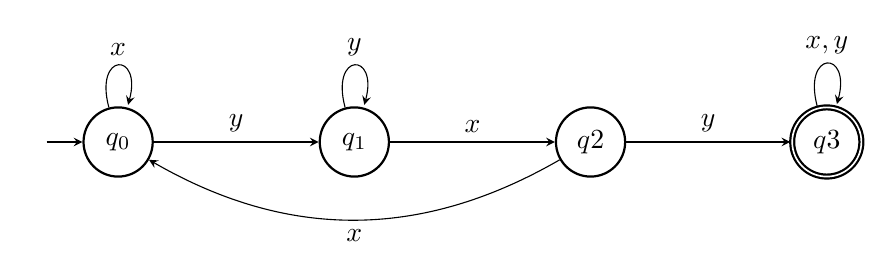
\begin{tikzpicture}
				\node[state, initial] (q0) {$q_0$};
				\node[state, right of=q0] (q1) {$q_1$};
				\node[state, right of=q1] (q2) {$q2$};
				\node[state, accepting, right of=q2] (q3) {$q3$};
				\draw	(q0) edge[loop above] node{$x$} (q0)
						(q0) edge[above] node{$y$} (q1)
						(q1) edge[loop above] node{$y$} (q1)
						(q1) edge[above] node{$x$} (q2)
						(q2) edge[bend left, below] node{$x$} (q0)
						(q2) edge[above] node{$y$} (q3)
						(q3) edge[loop above] node{$x, y$} (q3);
			\end{tikzpicture}
		\end{center}
		
		Cada estado representa lo sguiente:
		
		\begin{itemize}
			\item $q_0$ representa el estado inicial, y se continúa en él mientras le lleguen $x$, lo cuál significa
			que todavía no le ha llegado el primer elemento de la subcadena que debe contener.
			\item $q_1$ representa que ha llegado la primera $y$, y se mantiene en ese estado mientras sigan llegando
			$y$, ya que simboliza que al menos habrá una que forme parte de la cadena $yxy$. Se pasará al estado 
			$q_2$ cuando le llegue una $x$, que representa el elemento de en medio.
			\item $q_2$ representa que ha llegado la $x$ que forma la parte central de la cadena a aceptar. Si le llega
			una $x$ vuelve a $q_0$, ya que se ha interrumpido la cadena. Si le llega una $y$ significa que le ha llegado
			el último elemento de la cadena a aceptar y pasa al estado $q_3$.
			\item $q_3$ representa el estado final, al que se llega una vez que se han encontrado todos los símbolos
			consecutivos de la cadena. Se permanece en este estado le llegue lo que le llegue, ya que se ha encontrado
			la cadena que se buscaba. Si se llega a este estado, se acepta la cadena de entrada.
		\end{itemize}
		
		b) Definimos como Autómata Finito Determinista a la quintupla $M = (Q, A, q_0, \delta, F)$, donde $Q$ es
		el conjunto de estados, $A$ el alfabeto de entrada, $q_0$ el estado inicial, $\delta$ el conjunto de funciones
		de transición y $F$ el estado final. El autómata quedaría de la siguiente forma:
		
		\begin{center}
			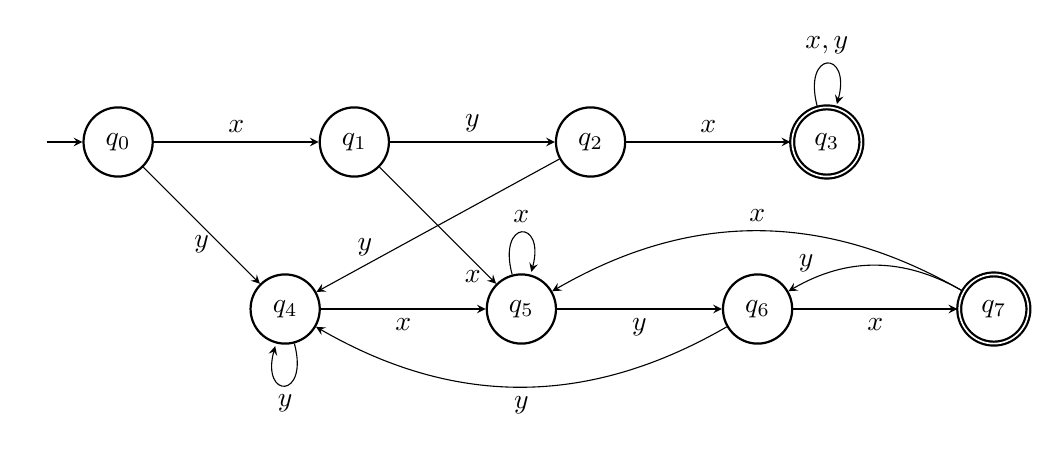
\begin{tikzpicture}
				\node[state, initial] (q0) {$q_0$};
				\node[state, right of=q0] (q1) {$q_1$};
				\node[state, right of=q1] (q2) {$q_2$};
				\node[state, accepting, right of=q2] (q3) {$q_3$};
				\node[state, below right of=q0] (q4) {$q_4$};
				\node[state, right of=q4] (q5) {$q_5$};
				\node[state, right of=q5] (q6) {$q_6$};
				\node[state, accepting, right of=q6] (q7) {$q_7$};
				\draw	(q0) edge[above] node{$x$} (q1)
						(q0) edge[below] node{$y$} (q4)
						(q1) edge[above] node{$y$} (q2)	
						(q1) edge[pos=0.8, below] node{$x$} (q5)
						(q2) edge[above] node{$x$} (q3)
						(q2) edge[pos=0.8, above] node{$y$} (q4)
						(q3) edge[loop above] node{$x, y$} (q3)
						(q4) edge[below] node{$x$} (q5)
						(q4) edge[loop below] node{$y$} (q4)
						(q5) edge[loop above] node{$x$} (q5)
						(q5) edge[below] node{$y$} (q6)
						(q6) edge[bend left, below] node{$y$} (q4)
						(q6) edge[below] node{$x$} (q7)
						(q7) edge[bend right, pos=0.9, above] node{$y$} (q6)
						(q7) edge[bend right, above] node{$x$} (q5);
			\end{tikzpicture}
		\end{center}
		
		Antes de explicar lo que representa cada estado, hace falta clarificar algunas ideas sobre el autómata.
		La parte de arriba del autómata representa el autómata capaz de aceptar las palabras que contienen la cadena
		$xyx$ al principio, mientras que la parte de abajo del autómata es la que es capaz de aceptar las palabras que
		contienen la cadena anterior al final de la palabra. Se aceptará una palabra si el autómata se encuentra en
		el estado $q_3$ o en el $q_7$ tras leer todos los símbolos de entrada. \par
		
		Una vez dicho esto, se 	va a proceder con la explicación:
		
		\begin{itemize}
			\item $q_0$ es el estado inicial. De aquí se pueden dar dos situaciones. La primera es que le llegue una
			$x$, lo cuál podría representar que la cadena $xyx$ se encuentra al principio de la palabra, y entonces
			se pasaría al estado $q_1$. En caso de que llegue una $y$, se descarta que la cadena se encuentre al
			principio de la palabra y se pasa al estado $q_4$ para intentar comprobar que se encuentra al final
			de la palabra.
			\item $q_1$ representa que ha llegado la primera $x$ y que se está comprobando que la cadena esté al
			principio. En caso de que le llegue una $y$ se pasará al estado $q_2$, esperando por tanto a que le llegue
			el último elemento. En caso de que le llegue una $x$, significa que la cadena a buscar no se pudo encontrar 
			al principio de la palabra y por tanto se intentará buscar al final de ésta. Por tanto, se pasará al estado
			$q_5$, simbolizando que ha llegado la primera $x$ que puede estar al final de la palabra.
			\item $q_2$ representa que han llegado los símbolos $xy$ al principio de la cadena y está esperando a que
			llegue la última $x$. En caso de que esto ocurra, se pasará al estado $q_3$. En caso de que llegue una $y$
			significaría que se está interrumpiendo la cadena al inicio y por tanto se pasaría al estado $q_4$,
			indicando que se intentará comprobar que la cadena está al final de la palabra, y que todavía no ha llegado
			el primer elemento de ésta.
			\item $q_3$ es un estado final que indica que se ha encontrado la cadena $xyx$ al principio de la palabra,
			y que por tanto se acepta la palabra. Ya que se ha cumplido la restricción, el autómata permanecerá en este
			estado sin importar que símbolo le venga de entrada.
			\item $q_4$ indica que, o bien el primer símbolo no ha sido una $x$ o que la cadena $xyx$ que se buscaba
			al principio o al final ha sido interrumpida con una $y$ (por ejemplo con la cadena $xyy$), y que por tanto 
			aun no ha llegado el primer elemento de la cadena a buscar. El autómata permanecerá en este estado mientras
			le siga llegando el símbolo $y$, y pasará al estado $q_5$ en cuanto le llegue una $x$, que simboliza el
			primer 	elemento de la cadena.
			\item $q_5$ representa un estado en el que se está buscando la cadena $xyx$ al final de la palabra y que
			ha llegado el primer elemento, bien porque la cadena había sido interrumpida por una $y$, como se ha
			mencionado en el estado anterior, o bien porque al principio ha llegado una cadena del tipo $xx$. Mientras
			le sigan llegando $x$, el autómata permanecerá en este estado, ya que este es el primer elemento de la
			cadena. Pasará a $q_6$ en cuánto le llegue el símbolo $y$.
			\item $q_6$ simboliza que se está buscando la cadena al final de la palabra y que de momento han llegado
			los símbolos $xy$. Si le llega el símbolo $y$, entonces se interrumpe la cadena, y se pasa al estado $q_4$.
			En caso de que llegue una $x$, el autómata pasará al estado $q_7$.
			\item $q_7$ representa es un estado final que indica que se ha encontrado la cadena $xyx$ al final de una
			palabra, probablemente. El autómata se quedará en este estado, y por tanto aceptará la palabra en el caso
			de que no le llegue ningún símbolo más. En caso de que le llegue una $x$, pasará al estado $q_5$,
			indicando que ha llegado el primer elemento de la cadena de nuevo. En caso de que le llegue una $y$,
			pasará al estado $q_6$, indicando que de momento lleva la cadena $xy$. Esto se debe a que anteriormente
			le llegó el símbolo $x$, con lo cuál, ahora con una $y$, lleva dos elementos de la cadena.
		\end{itemize}				
		
		c) Definimos como Autómata Finito Determinista a la quintupla $M = (Q, A, q_0, \delta, F)$, donde $Q$ es
		el conjunto de estados, $A$ el alfabeto de entrada, $q_0$ el estado inicial, $\delta$ el conjunto de funciones
		de transición y $F$ el estado final. El autómata quedaría de la siguiente forma:
		
		\begin{center}
			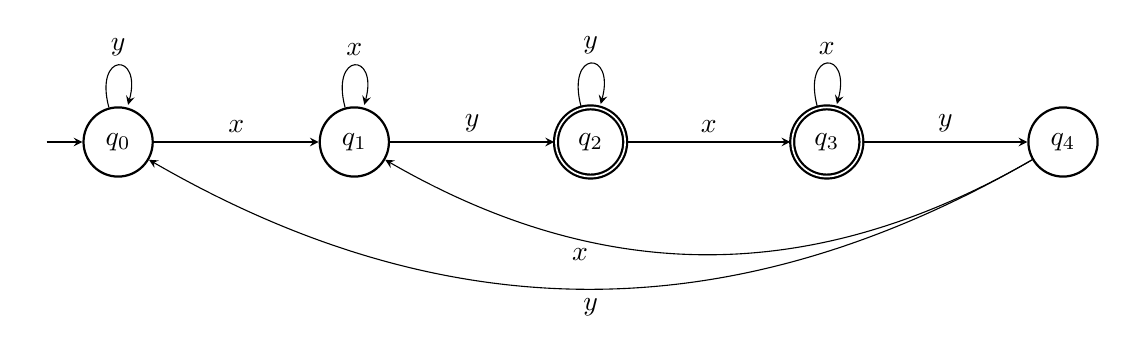
\begin{tikzpicture}
				\node[state, initial] (q0) {$q_0$};
				\node[state, right of=q0] (q1) {$q_1$};
				\node[state, accepting, right of=q1] (q2) {$q_2$};
				\node[state, accepting, right of=q2] (q3)  {$q_3$};
				\node[state, right of=q3] (q4) {$q_4$};
				\draw	(q0) edge[loop above] node{$y$} (q0)
						(q0) edge[above] node{$x$} (q1)
						(q1) edge[loop above] node{$x$} (q1)
						(q1) edge[above] node{$y$} (q2)
						(q2) edge[loop above] node{$y$} (q2)
						(q2) edge[above] node{$x$} (q3)
						(q3) edge[loop above] node{$x$} (q3)
						(q3) edge[above] node{$y$} (q4)
						(q4) edge[bend left, pos=0.7, below] node{$x$} (q1)
						(q4) edge[bend left, below] node{$y$} (q0);
			\end{tikzpicture}
		\end{center}
		
		Se va ahora a comentar cada estado:
		
		\begin{itemize}
			\item $q_0$ representa el estado inicial. El autómata se mantendrá en este estado mientras le sigan
			llegando símbolos $y$. Pasará al siguiente estado, $q_1$ cuando le llegue el símbolo $x$, el 	cuál forma
			parte de la cadena $xy$ a buscar.
			\item $q_1$ representa ha llegado el símbolo $x$ de la cadena $xy$. Se mantendrá en este estado
			mientras le sigan llegando síbolos $x$, ya que este sigue siendo el primer elemento de la cadena.
			Pasará al siguiente estado, $q_2$, en cuanto le llegue el símbolo $y$.
			\item $q_2$ es el primer estado final del autómata. Indica que se ha procesado la palabra y que se han
			encontrado un número impar de cadenas $xy$. Mientras le lleguen símbolos $y$, permanecerá en este estado.
			Por tanto, si el autómata está en este estado y no le llegan nuevos símbolos, o le siguen llegando $y$,
			aceptará la palabra.
			\item $q_3$ es el segundo estado final. Representa la situación en la que ha llegado un número de cadenas
			$xy$ impares y que ha llegado una nueva $x$, la cuál puede llegar a convertirse en una nueva cadena $xy$,
			haciendo que el número de éstas sea par. No obstante, como todavía no ha llegado un símbolo $y$, es un
			estado final, ya que como se mencionó anteriormente han llegado un número impar de cadenas $xy$. Por tanto,
			si el autómata se encuentra en este estado al finalizar de procesar la palabra, la aceptará. Se mantendrá
			en este estado mientras le sigan llegando símbolos $x$, y pasará al estado $q_4$ si le llega un símbolo $y$.
			\item $q_4$ es un estado que representa que han llegado un número par de cadenas $xy$. Si le llega un
			símbolo $y$ pasará al estado $q_0$. Si le llega una $x$, pasará al estado $q_1$, ya que se ha obtenido el
			primer símbolo de una potencial cadena $xy$.
		\end{itemize}
		
		
		\subsubsection{Ejercicio 2}
		\enu. En el alfabeto  $\lbrace 0, 1 \rbrace$, construir un AFND que acepte cada uno de los siguientes
		lenguajes:
		
		\begin{enumerate}[a)]
			\item El lenguaje de las palabras que empiezan en 1 y terminan en 010.
			\item El lenguaje de las palabras que empiezan o terminan (o ambas cosas) en 101.
			\item El lenguaje de las palabras que contienen, simultáneamente, las subcadenas 0101 y 100.
			El AFDN también acepta las cadenas en las que las subcadenas están solapadas (por ejemplo, ``10100” y
			``100101” serían palabras aceptadas).
		\end{enumerate}
		
		\sol \par
		
		a) Definimos como Autómata Finito No Determinista a la quintupla $M = (Q, A, q_0, \delta, F)$, donde $Q$ es
		el conjunto de estados, $A$ el alfabeto de entrada, $q_0$ el estado inicial, $\delta$ el conjunto de funciones
		de transición y $F$ el estado final. El autómata quedaría de la siguiente forma:
		
		\begin{center}
			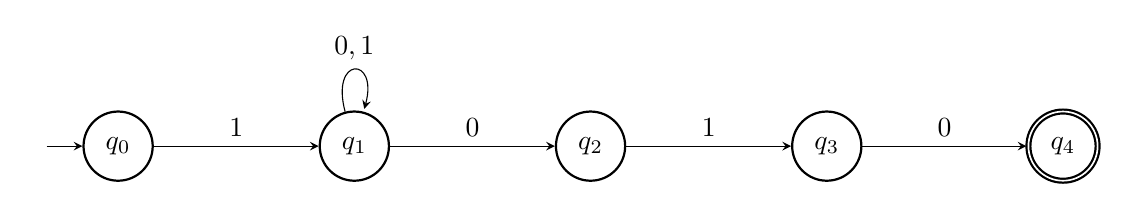
\begin{tikzpicture}
				\node[state, initial] (q0) {$q_0$};
				\node[state, right of=q0] (q1) {$q_1$};
				\node[state, right of=q1] (q2) {$q_2$};
				\node[state, right of=q2] (q3) {$q_3$};
				\node[state, accepting, right of=q3] (q4) {$q_4$};
				\draw	(q0) edge[above] node{$1$} (q1)
						(q1) edge[loop above] node{$0, 1$} (q1)
						(q1) edge[above] node{$0$} (q2)
						(q2) edge[above] node{$1$} (q3)
						(q3) edge[above] node{$0$} (q4);
			\end{tikzpicture}
		\end{center}
		
		A continuación, se va a explicar lo que representa cada estado:
		
		\begin{itemize}
			\item $q_0$ es el estado inicial. Desde él se pasa al estado $q_1$ en caso de que le llegue un 1 al principio
			de la palabra a procesar. En caso contrario, el autómata rechaza la palabra.
			\item $q_1$ representa que ya ha llegado un símbolo 1 como primer elemento de la palabra. Como se está trabajando
			con un AFND, el autómata estará en este estado mientras le sigan llegando 0 y 1, pero además transicionará al
			estado $q_2$ en cuanto le llega un 0.
			\item $q_2$ representa que ha llegado un 0 que potencialmente forma parte de la cadena 010 que se encuentra
			al final de la palabra. En caso de que le llegue un 1, el autómata pasaría al estado $q_3$. En caso de llegarle
			un 0, el autómata no sabría qué hacer y no pasaría a ningún estado. No obstante, ya que se mantiene al mismo
			tiempo en el estado $q_1$, el autómata permanecería en este estado y pasaría de nuevo al estado $q_2$.
			\item $q_3$ representa que ha llegado un 1 que potencialmente forma parte de la cadena 010 que se encuentra
			al final de una palabra. En caso de que le llegue un 0, el autómata transicionará al estado $q_4$. En caso
			de llegarle un símbolo 0, como no hay ninguna transición, el autómata no sabría que hacer y no haría nada.
			Sin embargo, como todavía se encuentra en el estado $q_1$, permanecería en este.
			\item $q_4$ es el estado final del autómata, y representa que le ha llegado una palabra con un 1 al principio
			y la cadena 010 al final. Por tanto, si al terminar de procesar una palabra el autómata se encuentra en este
			estado, se acepta la palabra. Esto es con la condición de que no le lleguen nuevos símbolos de entrada. Sin
			embargo, si le llegan, el autómata no sabrá que hacer, y por tanto dejará de aceptar la palabra. Sin embargo,
			como aún se mantiene en el estado $q_1$, hará alguna de las acciones especificadas para ese estado en función
			de la entrada.
		\end{itemize}
		
		b) Definimos como Autómata Finito No Determinista a la quintupla $M = (Q, A, q_0, \delta, F)$, donde $Q$ es
		el conjunto de estados, $A$ el alfabeto de entrada, $q_0$ el estado inicial, $\delta$ el conjunto de funciones
		de transición y $F$ el estado final. \par
		
		El autómata tiene dos partes: una para aceptar las palabras que contienen la cadena 101 al principio y una para
		aceptar las palabras que contienen 101 al final. Primero se procederá a mostrar el autómata que acepta las
		palabras que contienen la cadena al principio, el cuál quedaría de la siguiente forma:
		
		
		\begin{center}
			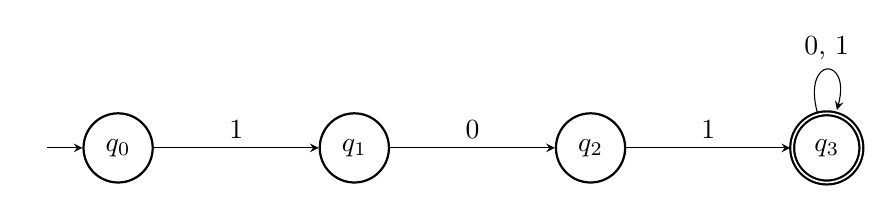
\begin{tikzpicture}
				\node[state, initial] (q0)  {$q_0$};
				\node[state, right of=q0] (q1) {$q_1$};
				\node[state, right of=q1] (q2) {$q_2$};
				\node[state, accepting, right of=q2] (q3) {$q_3$};
				\draw	(q0) edge[above] node{1} (q1)
						(q1) edge[above] node{0} (q2)
						(q2) edge[above] node{1} (q3)
						(q3) edge[loop above] node{0, 1} (q3);				
			\end{tikzpicture}
		\end{center}
		
		Como se puede ver, el autómata rechazará cualquier palabra que no empiece por 101, ya que en las transiciones
		no se especifica que hacer cuando le llegue un símbolo que no se espere. Una vez encontrada la cadena, da igual
		qué símbolo le llegue, ya que habrá cumplido el objetivo inicial. \par
		
		A continuación se va a construir el autómata que acepte las palabras que terminen en la secuencia 101:
		
		\begin{center}
			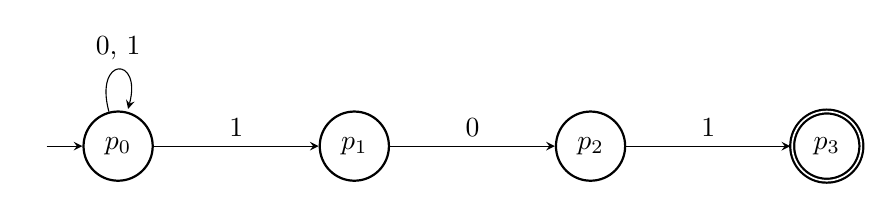
\begin{tikzpicture}
				\node[state, initial] (p0)  {$p_0$};
				\node[state, right of=p0] (p1) {$p_1$};
				\node[state, right of=p1] (p2) {$p_2$};
				\node[state, accepting, right of=p2] (p3) {$p_3$};
				\draw	(p0) edge[loop above] node{0, 1} (p0)
						(p0) edge[above] node{1} (p1)
						(p1) edge[above] node{0} (p2)
						(p2) edge[above] node{1} (p3);			
			\end{tikzpicture}
		\end{center}
		
		Como se puede comprobar fácilmente, este autómata procesa las palabras y las acepta si contienen la cadena 101 al
		final, es decir, si llega al estado $p_3$ y se mantiene ahí, sin que le llegue ningún símbolo nuevo. \par
		
		Para crear el autómata que acepta a la palabras que comiencen en 101 o acaben en 101, o ambas cosas, lo único que
		se tiene que hacer es unir los dos autómatas en uno mediante transiciones nulas. El resultado sería el siguiente:
		
		\begin{center}
			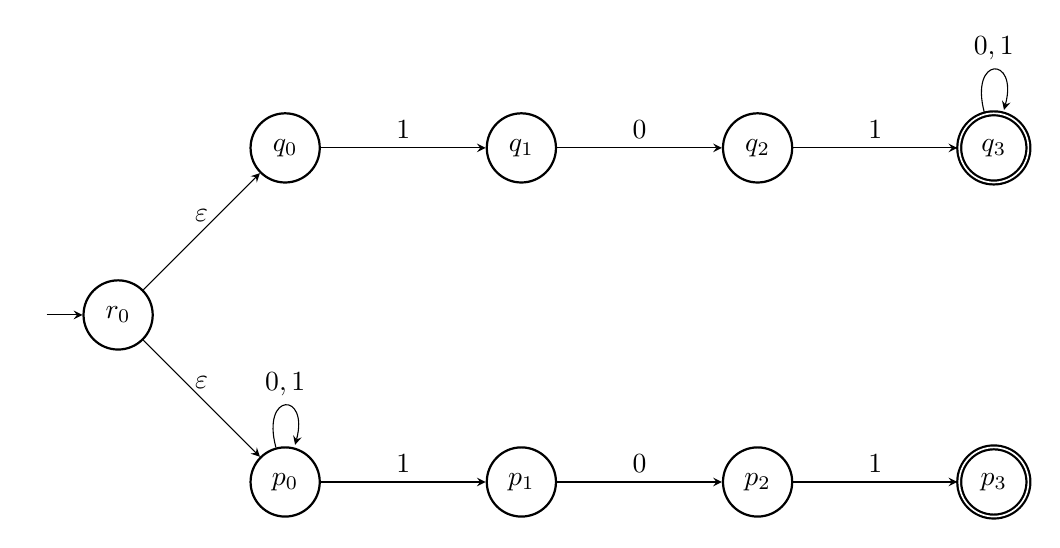
\begin{tikzpicture}
				\node[state, initial] (r0) {$r_0$};
				\node[state, above right of=r0] (q0)  {$q_0$};
				\node[state, right of=q0] (q1) {$q_1$};
				\node[state, right of=q1] (q2) {$q_2$};
				\node[state, accepting, right of=q2] (q3) {$q_3$};
				\node[state, below right of=r0] (p0)  {$p_0$};
				\node[state, right of=p0] (p1) {$p_1$};
				\node[state, right of=p1] (p2) {$p_2$};
				\node[state, accepting, right of=p2] (p3) {$p_3$};
				\draw	(r0) edge[above] node{$\varepsilon$} (q0)
						(q0) edge[above] node{1} (q1)
						(q1) edge[above] node{0} (q2)
						(q2) edge[above] node{1} (q3)
						(q3) edge[loop above] node{$0, 1$} (q3)
						(r0) edge[above] node{$\varepsilon$} (p0)
						(p0) edge[loop above] node{$0, 1$} (p0)
						(p0) edge[above] node{1} (p1)
						(p1) edge[above] node{0} (p2)
						(p2) edge[above] node{1} (p3);
			\end{tikzpicture}
		\end{center}
		
		Para que el autómata acepte una palabra de entrada, al terminar de procesarla debe encontrarse o bien en $q_3$,
		o bien en $p_3$, o bien en ambos estados.
		
		c) Definimos como Autómata Finito No Determinista a la quintupla $M = (Q, A, q_0, \delta, F)$, donde $Q$ es
		el conjunto de estados, $A$ el alfabeto de entrada, $q_0$ el estado inicial, $\delta$ el conjunto de funciones
		de transición y $F$ el estado final. \par
		
		El autómata tiene 2 partes: una que se encarga de comprobar que la palabra contenga las dos cadenas en el orden
		0101 y 100 y la otra que se encarga de comprobar que contiene las cadenas en el orden 100 y 0101. Ambas aceptan
		cadenas solapadas. \par
		
		Antes de empezar, vamos a construir los autómtas que aceptan cada cadena por separado, empezando por el que acepta
		las palabras que contengan la cadena 0101:
		
		\begin{center}
			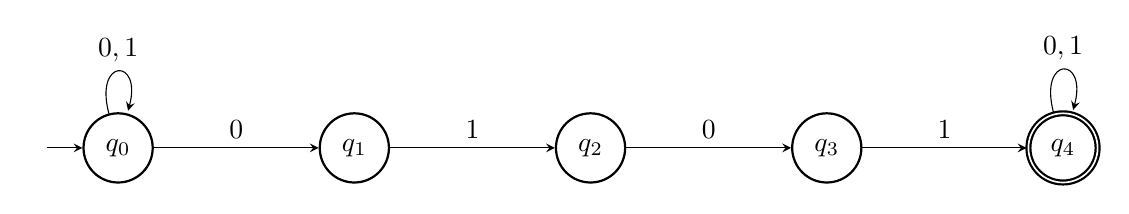
\begin{tikzpicture}
				\node[state, initial] (q0) {$q_0$};
				\node[state, right of=q0] (q1) {$q_1$};
				\node[state, right of=q1] (q2) {$q_2$};
				\node[state, right of=q2] (q3) {$q_3$};
				\node[state, accepting, right of=q3] (q4) {$q_4$};
				\draw	(q0) edge[loop above] node{$0, 1$} (q0)
						(q0) edge[above] node{0} (q1)
						(q1) edge[above] node{1} (q2)
						(q2) edge[above] node{0} (q3)
						(q3) edge[above] node{1} (q4)
						(q4) edge[loop above] node{$0, 1$} (q4);
			\end{tikzpicture}
		\end{center}
		
		Se puede comprobar fácilmente que este autómata procesa la palabra y busca en ella la cadena 0101, y la acaba
		aceptando si llega al estado $q_4$, una vez encontrada ésta. Al llegar a este estado, como se ha cumplido la
		restricción, da igual qué símbolo le llegue, ya que se mantendrá en el estado final. \par
		
		A continuación se muestra el autómata que busca la cadena 100:
		
		\begin{center}
			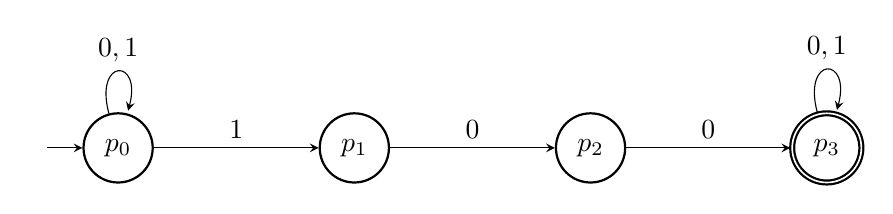
\begin{tikzpicture}
				\node[state, initial] (p0) {$p_0$};
				\node[state, right of=p0] (p1) {$p_1$};
				\node[state, right of=p1] (p2) {$p_2$};
				\node[state, accepting, right of=p2] (p3) {$p_3$};
				\draw	(p0) edge[loop above] node{$0, 1$} (p0)
						(p0) edge[above] node{1} (p1)
						(p1) edge[above] node{0} (p2)
						(p2) edge[above] node{0} (p3)
						(p3) edge[loop above] node{$0, 1$} (p3);
			\end{tikzpicture}
		\end{center}
		
		De nuevo, es fácil comprobar que el autómata procesa la palabra y determina si la cadena 100 forma parte de ella,
		aceptando la palabra de entrada si llega al estado $p_3$. Como da igual que símbolo de entrada le llegue una vez
		encontrada la cadena se mantendrá en ese estado final. \par
		
		Una vez dicho esto, se va a construir el autómata que acepte las palabras que contengan las cadenas 0101 y 100 en
		cualquier orden, y de ser el caso, solapadas. El autómata sería el siguiente:
		
		\begin{center}
			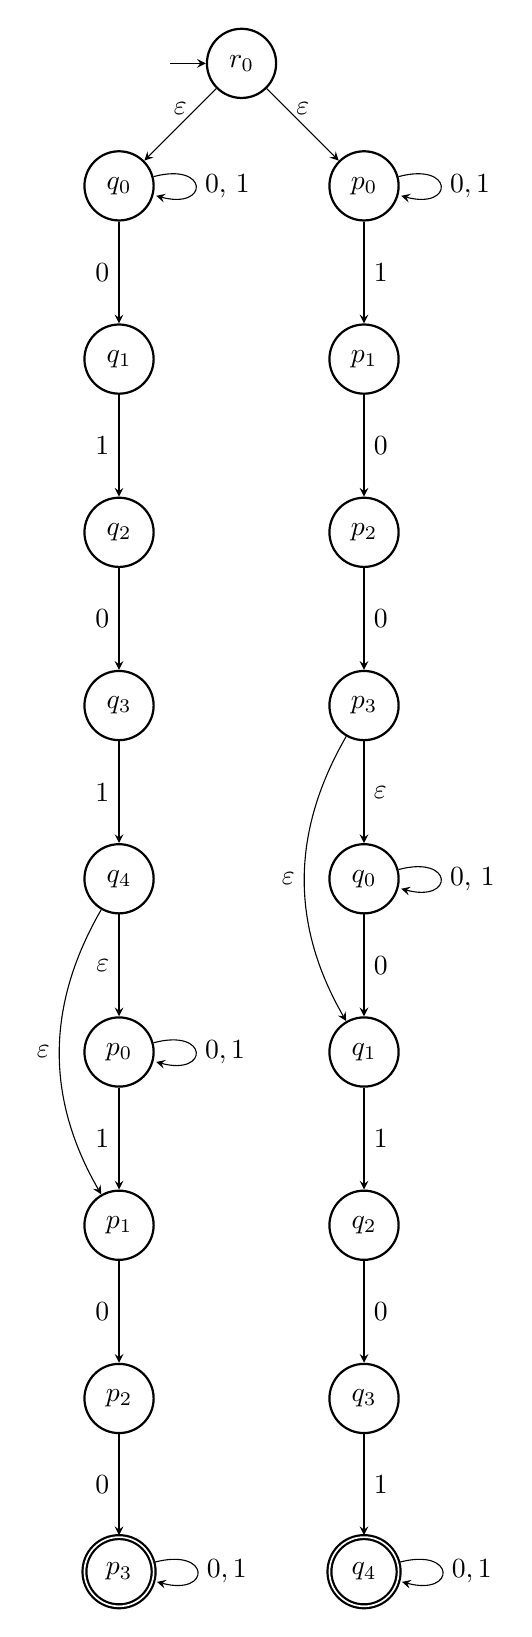
\begin{tikzpicture}[node distance=2.2cm]
				\node[state, initial] (r0) {$r_0$};
				
				\node[state, below left of=r0] (q0) {$q_0$};
				\node[state, below of=q0] (q1) {$q_1$};
				\node[state, below of=q1] (q2) {$q_2$};
				\node[state, below of=q2] (q3) {$q_3$};
				\node[state, below of=q3] (q4) {$q_4$};
				\node[state, below of=q4] (p0) {$p_0$};
				\node[state, below of=p0] (p1) {$p_1$};
				\node[state, below of=p1] (p2) {$p_2$};
				\node[state, accepting, below of=p2] (p3) {$p_3$};
				
				\node[state, below right of=r0] (p4) {$p_0$};
				\node[state, below of=p4] (p5) {$p_1$};
				\node[state, below of=p5] (p6) {$p_2$};
				\node[state, below of=p6] (p7) {$p_3$};
				\node[state, below of=p7] (q5) {$q_0$};
				\node[state, below of=q5] (q6) {$q_1$};
				\node[state, below of=q6] (q7) {$q_2$};
				\node[state, below of=q7] (q8) {$q_3$};
				\node[state, accepting, below of=q8] (q9) {$q_4$};
				
				\draw	(r0) edge[above] node{$\varepsilon$} (q0)
						(q0) edge[loop right] node{0, 1} (q0)
						(q0) edge[left] node{0} (q1)
						(q1) edge[left] node{1} (q2)
						(q2) edge[left] node{0} (q3)
						(q3) edge[left] node{1} (q4)
						(q4) edge[left] node{$\varepsilon$} (p0)
						(p0) edge[loop right] node{$0, 1$} (p0)
						(p0) edge[left] node{1} (p1)
						(p1) edge[left] node{0} (p2)
						(p2) edge[left] node{0} (p3)
						(p3) edge[loop right] node{$0, 1$} (p3)
						(q4) edge[bend right, left] node{$\varepsilon$} (p1)
						(r0) edge[above] node{$\varepsilon$} (p4)
						(p4) edge[loop right] node{$0, 1$} (p4)
						(p4) edge[right] node{1} (p5)
						(p5) edge[right] node{0} (p6)
						(p6) edge[right] node{0} (p7)
						(p7) edge[right] node{$\varepsilon$} (q5)
						(q5) edge[loop right] node{0, 1} (q5)
						(q5) edge[right] node{0} (q6)
						(q6) edge[right] node{1} (q7)
						(q7) edge[right] node{0} (q8)
						(q8) edge[right] node{1} (q9)
						(q9) edge[loop right] node{$0, 1$} (q9)
						(p7) edge[bend right, left] node{$\varepsilon$} (q6);
			\end{tikzpicture}
		\end{center}
		
		Para que se solapen las cadenas, se han añadido transiciones nulas que permiten pasar de la parte final de un
		autómata al estado siguiente del inicial del otro. Adicionalmente, entre el final de un autómata y el principio
		del otro se han añadido transiciones nulas para conectarlos. \par
		
		El autómata aceptará las palabras si llega a uno de los dos estados finales del autómata. Como son mutuamente
		excluyentes, solo puede llegar a uno. 
			
		\subsubsection{Ejercicio 3}
		\enu. Calcular una máquina de Mealy o Moore que codifique el complemento a dos de un número en binario. \par
		\textbf{\underline{Nota}}: \textit{El complemento a dos se realiza cambiando ceros por unos y unos por ceros, y
		luego, al resultado, sumándole uno en binario.} \par
		\textbf{\underline{Nota 2}}: \textit{El complemento a dos es la forma en que se calcula el entero opuesto a uno
		dado para la representación binaria de los enteros con signo en C++.} \par
		
		\sol \par
		
		Se va a construir una máqiona de Mealy que permita calcular el complemento a dos de un número binario. En esta
		máquina, las salidas correspondientes a las entradas se indican en las transiciones en vez de en los estados en
		sí. \par
		
		El resultado sería el siguiente:
		
		\begin{center}
			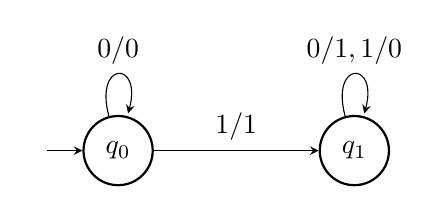
\begin{tikzpicture}
				\node[state, initial] (q0) {$q_0$};
				\node[state, right of=q0] (q1) {$q_1$};
				\draw	(q0) edge[loop above] node{$0/0$} (q0)
						(q0) edge[above] node{$1/1$} (q1)
						(q1) edge[loop above] node{$0/1, 1/0$} (q1);
			\end{tikzpicture}
		\end{center}
		
		El comportamiento del autómata sería el siguiente:
		
		\begin{itemize}
			\item Si el primer elemento de entrada es un 0, y mientras le sigan llegando símbolos 0, el autómata imprimirá
			el símbolo 0. Esto se debe a que al dígito más a la derecha se le suma un 1 en el complemento a 2. Por tanto,
			si el complemento a 1 de 0 es 1, y al sumarle el 1 del complemento a 2, su valor pasa a ser 0, y se tiene un 1 de
			acarreo, el cuál se sumará al siguiente símbolo de entrada. Si vuelve a entrar un 0, se obtiene un 1 del
			complemento a 1 y se le suma el acarreo, produciendo un 0 de nuevo con acarreo, y así sucesivamente. En el
			autómata esto se representa con el estado $q_0$ y la transición que sale y entra hacia él.
			\item Si el primer símbolo es 1, o llega el primer 1 de la cadena, se le hace su complemento a 1, el cuál es 0,
			y se le suma un 1 si es el primer elemento de entrada o si han llegado anteriormente símbolos 0 y se ha producido
			acarreo, resultando por tanto en 1. En este caso, no se produciría acarreo, y los símbolos que vengan a
			continuación tendrán su valor inverso. Esto se representa con la transición de $q_0$ a $q_1$.
			\item Una vez que ya no hay acarreo y sigan llegando símbolos de entrada, se imprimirá el valor contrario al de
			entrada. Por ejemplo, si llega un 0 se imprimirá un 1, y si llega un 1, un 0. Esto se representa con la transición
			que entra y sale de $q_1$.
		\end{itemize}						
		
		\subsubsection{Ejercicio 4}
		\enu. Diseñar una Máquina de Mealy o de Moore que, dada una cadena usando el alfabeto $A = \lbrace a, w, o
		\rbrace$, encienda un led verde (salida $V$) cada vez que se detecte la cadena ``$woow$" en la entrada,
		apagándolo cuando lea cualquier otro símbolo después de esta cadena (representamos el led apagado con la
		salida ``$X$"). El autómata tiene que encender el led verde (salida $V$), tantas veces como aparezca en la
		secuencia ``$woow$" en la entrada, y esta secuencia puede estar solapada \par
	
		\sol \par
		
		Se plantea una máquina de Mealy como solución al problema dado, la cuál tiene la siguiente forma:
		
		\begin{center}
			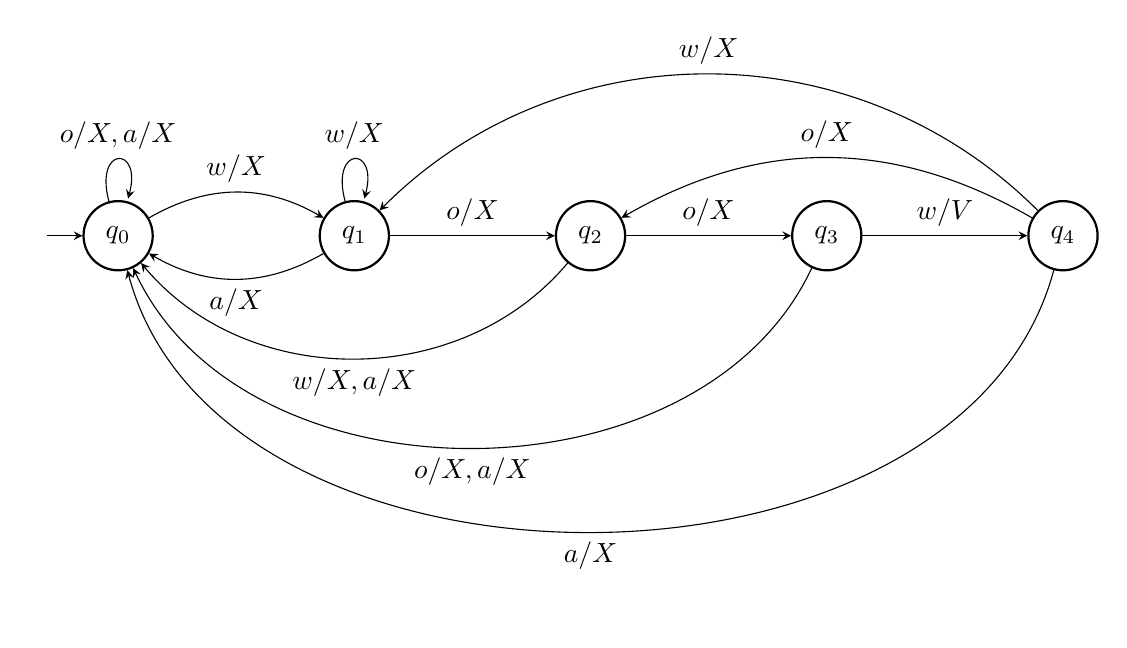
\begin{tikzpicture}
				\node[state, initial] (q0) {$q_0$};
				\node[state, right of=q0] (q1) {$q_1$};
				\node[state, right of=q1] (q2) {$q_2$};
				\node[state, right of=q2] (q3) {$q_3$};
				\node[state, right of=q3] (q4) {$q_4$};
				\draw	(q0) edge[loop above] node{$o/X, a/X$} (q0)
						(q0) edge[bend left, above] node{$w/X$} (q1)
						(q1) edge[bend left, below] node{$a/X$} (q0)
						(q1) edge[loop above] node{$w/X$} (q1)
						(q1) edge[above] node{$o/X$} (q2)
						(q2) edge[above] node{$o/X$} (q3)
						(q3) edge[above] node{$w/V$} (q4)
						
						(q2) edge[bend left=50, below] node{$w/X, a/X$} (q0)
						(q3) edge[bend left=65, below] node{$o/X, a/X$} (q0)
						(q4) edge[bend left=75, below] node{$a/X$} (q0)
						(q4) edge[bend right=45, above] node{$w/X$} (q1)
						(q4) edge[bend right, above] node{$o/X$} (q2);
			\end{tikzpicture}		
		\end{center}
		
		A continuación se va a explicar brevemente el funcionamiento de la máquina:
		
		\begin{itemize}
			\item $q_0$ es el estado inicial y al que transicionan todos los estados cuando les llega un símbolo que no
			esperaban. Representa además un estado en el que todavía no ha llegado ningún elemento de la cadena ``$woow$".
			\item $q_1$ representa el estado siguiente de $q_0$, en el cuál le llega la primera $w$. Mientras le sigan
			llegando $w$ permanecerá en este estado, ya que sigue siendo el primer elemento de la cadena. Cuando le llegue
			una $o$ pasará al siguiente estado.
			\item $q_2$ representa que ha llegado la primera $o$, y si le llega cualquier otro elemento que no sea otra
			$o$, vuelve al estado $q_0$. En caso de que le llegue, pasa al siguiente estado.
			\item $q_3$ representa un estado en el que han llegado las dos $o$ y está esperando una $w$ para pasar al
			siguiente estado y encender finalmente el led de color verde. En caso de llegarle otro símbolo, volverá al 
			estado $q_0$.
			\item $q_4$ representa que han llegado todos los elementos de la cadena ``$woow$" y que se ha encendido el led
			verde (mediante la transición $w/X$ para pasar de $q_3$ a $q_4$). Desde aquí, como se pueden solapar las
			cadenas, pueden darse distintas situaciones. La primera es que le llegue una $a$, pasando por tanto al estado
			$q_0$. Si le llega una $w$, significa que puede llegar una nueva cadena ``$woow$" sin solapar, y por tanto pasará
			al estado $q_1$, simbolizando que ha llegado la primera $w$. En caso de llegarle una $o$, significa que
			posiblemente la cadena se solape, pasando por tanto al estado $q_2$, indicando que ha llegado la primera $o$.
		\end{itemize}
		
	\newpage
	\subsection{Práctica 4}
	
		\subsubsection{Ejercicio 1}
		\enu. Dado el siguiente autómata responde a las siguientes cuestiones razonadamente:
		
		\begin{enumerate}[a)]
			\item ¿Habría alguna forma de optimizar el autómata para que reduciendo su complejidad siga aceptado exactamente
			el mismo lenguaje?
			\item ¿Se podría obtener la gramática que genera este lenguaje en la Forma Normal de Chomsky? En caso afirmativo,
			proporcionar dicha gramática en FNC. En caso contrario, justificar.
		\end{enumerate}
		
		\begin{center}
			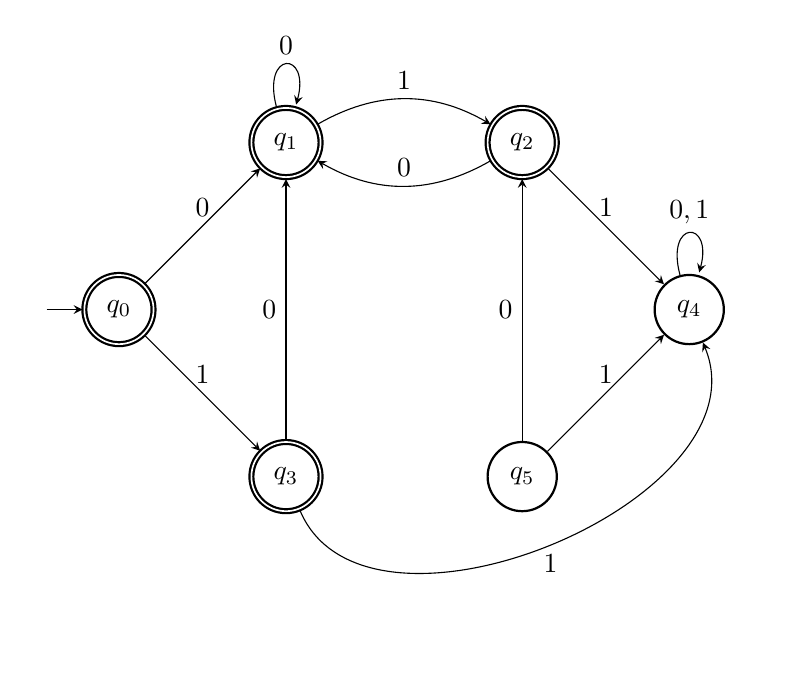
\begin{tikzpicture}
			\node[state, initial, accepting] (q0) {$q_0$};
			\node[state, accepting, above right of=q0] (q1) {$q_1$};
			\node[state, accepting, right of=q1] (q2) {$q_2$};
			\node[state, accepting, below right of=q0] (q3) {$q_3$};
			\node[state, below right of=q2] (q4) {$q_4$};
			\node[state, right of=q3] (q5) {$q_5$};
			\draw	(q0) edge[above] node{$0$} (q1)
					(q0) edge[above] node{$1$} (q3)
					(q1) edge[loop above] node{$0$} (q1)
					(q1) edge[bend left, above] node{$1$} (q2)
					(q2) edge[bend left, above] node{$0$} (q1)
					(q2) edge[above] node{$1$} (q4)
					(q3) edge[left] node{$0$} (q1)
					(q3) edge[bend right=90, below] node{$1$} (q4)
					(q4) edge[in=75, out=105, loop, above] node{$0, 1$} (q4)
					(q5) edge[left] node{$0$} (q2)
					(q5) edge[above] node{$1$} (q4)					
					;
			\end{tikzpicture}
		\end{center}
		
		\sol \par
		
		a) Para intentar optimizar el autómata y reducir su complejidad se puede aplicar el algoritmo de minimización. En
		caso de obtener el mismo autómata después de intentar minimizarlo, significaría que ya se estaría delante de un
		autómata minimal, y que por tanto no se puede simplificar más. \par
		
		Para empezar, se van a eliminar todos los estados inaccesibles, es decir, aquellos a los que no se pueda llegar
		desde ningún otro estado. \par
		
		Como se puede observar claramente, el estado $q_5$ es inaccesible, ya que no se puede llegar hasta él de ninguna
		forma. Dicho de otra manera, no existe ninguna transición que lleve cualquier estado a $q_5$. Por tanto se eliminaría,
		y el resultado sería el siguiente:
		
		\begin{center}
			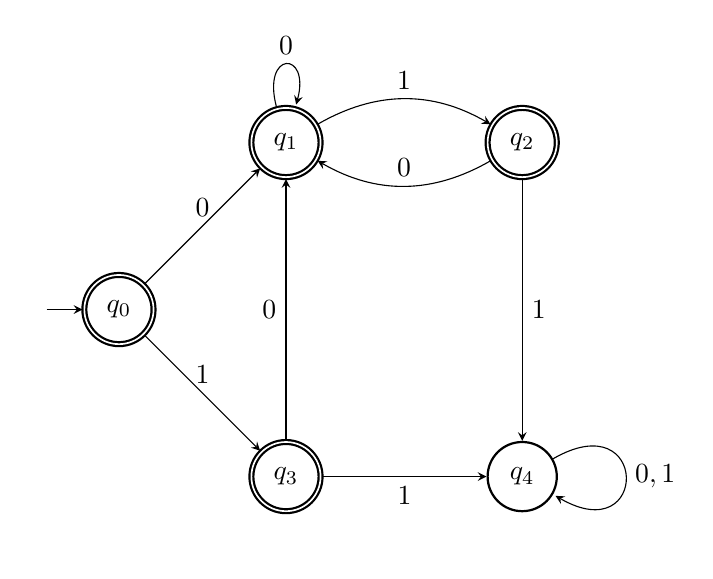
\begin{tikzpicture}
			\node[state, initial, accepting] (q0) {$q_0$};
			\node[state, accepting, above right of=q0] (q1) {$q_1$};
			\node[state, accepting, right of=q1] (q2) {$q_2$};
			\node[state, accepting, below right of=q0] (q3) {$q_3$};
			\node[state, right of=q3] (q4) {$q_4$};
			\draw	(q0) edge[above] node{$0$} (q1)
					(q0) edge[above] node{$1$} (q3)
					(q1) edge[loop above] node{$0$} (q1)
					(q1) edge[bend left, above] node{$1$} (q2)
					(q2) edge[bend left, above] node{$0$} (q1)
					(q2) edge[right] node{$1$} (q4)
					(q3) edge[left] node{$0$} (q1)
					(q3) edge[below] node{$1$} (q4)
					(q4) edge[in=-30, out=30, loop, right] node{$0, 1$} (q4)				
					;
			\end{tikzpicture}
		\end{center}
		
		Una vez eliminados los estados inaccesibles se puede aplicar el algoritmo de minimización. Con este algoritmo se
		intentan reducir el número de estados, dejando solo aquellos que son distinguibles entre sí. Dos estados son
		distinguibles si, para un mismo símbolo de entrada, se llegan a dos estados diferentes (es decir, que uno sea final
		y el otro no, por ejemplo). Si dos estados son distinguibles, significia que los estados padres también lo serán, ya
		que los hijos se pueden distinguir. Con esto se busca reducir el número de estados, combinando aquellas parejas que son
		indistinguibles en un solo estado.
		\par
		
		Para ello, se va a construir una tabla triangular y se van a marcar con una cruz las casillas en las que la pareja
		de estados sea distinguible. Se hará una primera iteración, en la que se marcarán aquellas parejas distinguibles sin
		que les entre ningún símbolo de entrada. Es decir, aquellas en las que uno de los estados sea final y el otro no. \par
		
		El resultado de esta primera iteración es el siguiente:
		
		\begin{center}
			\begin{tabular}{*{7}{c|}}
																							\cline{2-2}
				1 & 																		\\ \cline{2-3}
				2 & &																		\\ \cline{2-4}
				3 & & &																		\\ \cline{2-5}
				4 & \color{blue}{X} & \color{blue}{X} & \color{blue}{X} & \color{blue}{X}	\\ \cline{2-5}
				\multicolumn{0}{c}{} & \multicolumn{1}{c}{0} & \multicolumn{1}{c}{1} & \multicolumn{1}{c}{2}
				& \multicolumn{1}{c}{3}
			\end{tabular}
		\end{center}
		
		Como se puede observar, el estado $q_4$ es distinguible de todos los otros porque es el único que no es final. Los
		demás, de momento, son indistinguibles, así que se irán comprobando por partes a medida que se itere. El criterio
		a seguir ahora para determinar si dos estados son distinguibles es comprobar, según el símbolo de entrada, hacia
		donde transiciona cada pareja. En caso de llegar con cualquiera de los símbolos de entrada del lenguaje a una pareja
		de estados distinguibles, entonces se marcará en la tabla que esa pareja también lo es. En caso de ir a una pareja
		de estados que todavía no se ha marcado, se guardará la pareja y, si al comprobar la pareja a la que llegan se
		determina que esos valores son distinguibles, entonces también se marcará a la pareja original como distinguible.
		En caso contrario, no se hará nada. Este proceso, como se puede ver, determina recursivamente las parejas que son
		distinguibles, reduciendo por tanto el número de iteraciones que se tienen que hacer. \par
		
		A continuación, se van a comprobar las parejas formadas por el estado $q_3$ con los estados $q_0$, $q_1$ y $q_2$, ya
		que todavía no se ha determinado si son distinguibles estas parejas. Para eso, se van a construir tablas que permitan
		ver hacia donde se transiciona con las entradas. Se marcarán en rojo aquellas transiciones que ya sean distinguibles
		para facilitar el seguimiento del algoritmo. Luego se mostrará el resultado en la tabla donde se minimiza. \par
		
		Este es el resultado para las parejas mencionadas anteriormente:
		
		\begin{figure}[H]
			\centering
			\begin{tabular}{c|cc}
				& 0 & 1		\\ \hline
				0 & 1 & \color{red}{3}	\\
				3 & 1 & \color{red}{4}	\\ \hline
				1 & 1 & \color{red}{2}	\\ 
				3 & 1 & \color{red}{4}	\\ \hline
				2 & 1 & 4	\\
				3 & 1 & 4	\\ \hline				
			\end{tabular}
		\end{figure}
		
		\begin{figure}[H]
			\centering
			\begin{tabular}{*{7}{c|}}
																							\cline{2-2}
				1 & 																		\\ \cline{2-3}
				2 & &																		\\ \cline{2-4}
				3 & \color{red}{X} & \color{red}{X} &										\\ \cline{2-5}
				4 & \color{blue}{X} & \color{blue}{X} & \color{blue}{X} & \color{blue}{X}	\\ \cline{2-5}
				\multicolumn{0}{c}{} & \multicolumn{1}{c}{0} & \multicolumn{1}{c}{1} & \multicolumn{1}{c}{2}
				& \multicolumn{1}{c}{3}
			\end{tabular}
		\end{figure}
		
		Como se puede comprobar, solo la pareja $\lbrace q_2, q_3 \rbrace$ ha quedado sin marcar, y tampoco parece llegar
		a ningún estado que pueda ser comprobado más adelante. Con lo cuál, como a medida que se itere no se volverá atrás,
		se puede decir de momento que la pareja $\lbrace q_2, q_3 \rbrace$ es indistinguible. \par
		
		Ahora se procederá a comprobar el estado $q_2$ con los estados $q_0$ y $q_1$. El resultado es el siguiente:
		
		\begin{figure}[H]
			\centering
			\begin{tabular}{c|cc}
				& 0 & 1		\\ \hline
				0 & 1 & \color{red}{3}	\\
				2 & 1 & \color{red}{4}	\\ \hline
				1 & 1 & \color{red}{2}	\\ 
				2 & 1 & \color{red}{4}	\\ \hline				
			\end{tabular}
		\end{figure}
		
		\begin{figure}[H]
			\centering
			\begin{tabular}{*{7}{c|}}
																							\cline{2-2}
				1 & 																		\\ \cline{2-3}
				2 & \color{red}{X} & \color{red}{X}											\\ \cline{2-4}
				3 & \color{red}{X} & \color{red}{X} &										\\ \cline{2-5}
				4 & \color{blue}{X} & \color{blue}{X} & \color{blue}{X} & \color{blue}{X}	\\ \cline{2-5}
				\multicolumn{0}{c}{} & \multicolumn{1}{c}{0} & \multicolumn{1}{c}{1} & \multicolumn{1}{c}{2}
				& \multicolumn{1}{c}{3}
			\end{tabular}
		\end{figure}
		
		Aquí se puede ver que todas las parejas de estados posibles son distinguibles con $q_2$, por tanto se han marcado
		las casillas que corresponden en la tabla. \par
		
		Para finalizar se va a comprobar la pareja formada por los estados $q_0$ y $q_1$. El resultado es el siguiente:
		
		\begin{figure}[H]
			\centering
			\begin{tabular}{c|cc}
				& 0 & 1		\\ \hline
				0 & 1 & 3	\\
				1 & 1 & 2	\\ \hline				
			\end{tabular}
		\end{figure}
		
		\begin{figure}[H]
			\centering
			\begin{tabular}{*{7}{c|}}
																							\cline{2-2}
				1 & 																		\\ \cline{2-3}
				2 & \color{red}{X} & \color{red}{X}											\\ \cline{2-4}
				3 & \color{red}{X} & \color{red}{X} &										\\ \cline{2-5}
				4 & \color{blue}{X} & \color{blue}{X} & \color{blue}{X} & \color{blue}{X}	\\ \cline{2-5}
				\multicolumn{0}{c}{} & \multicolumn{1}{c}{0} & \multicolumn{1}{c}{1} & \multicolumn{1}{c}{2}
				& \multicolumn{1}{c}{3}
			\end{tabular}
		\end{figure}
		
		Después de esta última iteración se ha concluído que la pareja de estados $\{q_0, q_1\}$ también son indistinguibles,
		ya que no conducen a ningún estado distinguible. \par
		
		Por tanto, se puede afirmar que las parejas de estados $\{q_0, q_1\}$ y $\{q_2, q_3\}$ son indistinguibles. Esto
		implica que los dos estados se pueden juntar en uno nuevo, conservando las transiciones de ambos estados. \par
		
		Para finalizar, se va a crear el nuevo autómata, el cuál es mínimo y el más simple posible, con las agrupaciones
		de estados correspondientes. El resultado sería el siguiente:
		
		\begin{figure}[H]
			\centering
			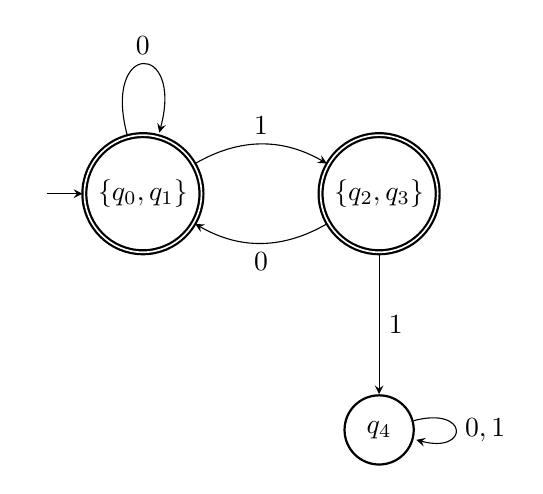
\begin{tikzpicture}
			\node[state, initial, accepting] (q01) {$\{q_0, q_1\}$};
			\node[state, accepting, right of=q01] (q23) {$\{q_2, q_3\}$};
			\node[state, below of=q23] (q4) {$q_4$};
			\draw	(q01) edge[loop above] node{$0$} (q01)
					(q01) edge[bend left, above] node{$1$} (q23)
					(q23) edge[bend left, below] node{$0$} (q01)
					(q23) edge[right] node{$1$} (q4)
					(q4) edge[loop right] node{$0, 1$} (q4)				
					;
			\end{tikzpicture}
		\end{figure}
		
		b) Lo primero que se va a hacer es pasar el AFD anterior a gramática. Definimos gramática como la cuádrupla $G = (V,
		T, P, S)$, donde $V$ son las variables, $T$ los símbolos terminales, $P$ el conjunto de reglas de producción y $S$
		el estado inicial. Para facilitar el trabajo se va a nombrar al estado $\{q_0, q_1\}$ como $S$, al $\{q_2, q_3\}$
		como $A$ y al estado $q_4$ como $B$. Por tanto, la gramática sería la siguiente:
		
		\[V = \{S, A, B\}\]
		\[T = \{0, 1\}\]
		\[P = \{S \rightarrow 0S \; | \; 1A \; | \; \varepsilon, \; A \rightarrow 0S \; | \; 1B \; | \; \varepsilon, \;
				B \rightarrow 0B \; | \; 1B\} \]
		\[S = \{ S \} \]
		
		La Forma Normal de Chomsky tiene las reglas de producción de la forma $A \rightarrow BC$ y $A \rightarrow a$, donde
		$A, B, C \in V$ y $a \in T$. Como se puede ver, nuestra gramática se encuentra lejos de eso. \par
		
		El primer paso consiste en limpiar la gramática de producciones inútiles, es decir, de las variables que no produzcan
		un símbolo terminal y de aquellas variables inalcanzables. Al limpiar la gramática anterior, obtenemos la siguiente:
		
		\[V = \{S, A\}\]
		\[T = \{0, 1\}\]
		\[P = \{S \rightarrow 0S \; | \; 1A \; | \; \varepsilon, \; A \rightarrow 0S \; | \; \varepsilon\} \]
		\[S = \{ S \} \]	
		
		Como se puede ver, la variable $B$ ha sido eliminada, ya que no producía ningún símbolo terminal. \par
		
		Una vez limpiada la gramática, el siguiente paso consiste en eliminar las producciones nulas y sustituirlas por
		los símbolos terminales que correspondan. Las reglas de producción, una vez aplicado este paso, quedarían de la
		siguiente forma:
		
		\[P = \{S \rightarrow 0S \; | \; 1A \; | \; 0 \; | \; 1, \; A \rightarrow 0S \; | \; 0\} \]
		
		Como se puede ver, ahora nuestra gramática no contiene producciones nulas, y se puede pasar al paso final, que
		consiste en dejar todas las producciones de la forma $A \rightarrow BC$ y $A \rightarrow a$, donde $A, B, C \in V$
		y $a \in T$. Una vez aplicado el proceso de transformación de la gramática, obtenemos la siguiente gramática, la
		cuál ya está en la Forma Normal de Chomsky:
		
		\[V = \{S, A, X, Y\}\]
		\[T = \{0, 1\}\]
		\[P = \{X \rightarrow 0, \; Y \rightarrow 1, \; S \rightarrow XS \; | \; YA \; | \; 0 \; | \; 1, \;
				A \rightarrow XS \; | \; 0\} \]
		\[S = \{ S \} \]
		
		Como se puede comprobar fácilmente, todas las producciones siguen las condiciones descritas anteriormente. El proceso
		para llegar hasta esta gramática ha consistido en sustituir en las reglas de producción los símbolos terminales que
		iban acompañados por una variable por otra variable (cambiar $0$ y $1$ por $X$ e $Y$, respectivamente). Esa variable
		luego se sustituye por el símbolo terminal correspondiente. Si una regla producía un símbolo terminal, no se ha
		cambiado el símbolo por la nueva variable, solo en los casos en los que va acompañado de otra variable.
		
		\subsubsection{Ejercicio 2}
		\enu. Observando las siguientes gramáticas, determinar cuáles de ellas son ambiguas y, en su caso, comprobar si los
		lenguajes generados son inherentemente ambiguos. Justificar la respuesta.
		
		\begin{enumerate}[a)]
			\item $S \rightarrow AbB, \; A \rightarrow aA \; | \; \varepsilon, \; B \rightarrow aB \; | \; bB \; | \;
			\varepsilon$
			\item $S \rightarrow abaS \; | \; babS  \; | \; baS \; | \; \varepsilon$
			\item $S \rightarrow aSA \; | \; \varepsilon, \; A \rightarrow bA \; | \; \varepsilon$
		\end{enumerate}
		
		\textit{\underline{Nota}: Explicar y demostrar cuidadosamente si la gramática no es ambigua (con lenguaje natural).}
		
		\sol \par
		
		a) La gramática no es ambigua. En un principio puede parecerlo ya que al principio, con la regla $S \rightarrow AbB$
		se crea un árbol que puede crecer tanto por la derecha como por la izquierda. Sin embargo, el resto de reglas obligan
		a crecer esas ramas obligatoriamente hacia la derecha. Aunque en un principio eso no llega a salvar a la gramática de
		ser ambigua, en este caso no se produce ninguna ambigüedad. Esto se puede ver de la siguiente forma:
		
		\begin{itemize}
			\item En la parte derecha de la palabra habrá una sucesión de 0 o más símbolos $a$. Como los símbolos se van
			poniendo uno detrás de otro hasta que se inserte el símbolo vacío, solo hay camino único para un número dado
			de símbolos $a$.
			\item Entre las dos partes que pueden crecer del árbol siempre habrá un símbolo $b$.
			\item En la parte izquierda habrá 0 o más símbolos $a$ y $b$, entremezclados o no. La forma en la que va creciendo
			esta parte del árbol permite seguir un camino único para cada posible combinación de símbolos $a$ y $b$ que se
			genere, con lo cuál no es posible obtener dos árboles distintos para una misma sucesión de símbolos.
		\end{itemize}
		
		Al demostrar que la gramática no es ambigua, se puede decir también que el lenguaje no es inherentemente ambigua, ya
		que existe al menos una gramática no ambigua para éste.
		
		b)
		
		c) La gramática es ambigua, ya que se puede obtener la cadena $aab$ con dos árboles distintos, los cuáles son:
		\begin{figure}[H]
			\centering
			\begin{tikzpicture}[ -, xscale=0.8,
								level 1/.style={sibling distance=12em},
								level 2/.style={sibling distance=6em},
								level 3/.style={sibling distance=3em},
								level 4/.style={sibling distance=2em}]
				\node (S1) {$S$}
					child{
						node (a1) {$a$}
					}
					child{
						node (S2) {$S$}
						child { node (a2) {$a$} }
						child{
							node (S3) {$S$}
							child{ node (e1) {$\varepsilon$} }
						}
						child {
							node (A2) {$A$}
							child { node (b) {$b$} }
							child {
								node (A3) {$A$}
								child { node (e3) {$\varepsilon$} }
							}
						}
					}
					child {
						node (A1) {$A$}
						child { node (e2) {$\varepsilon$} }
					}					
					;
			\end{tikzpicture}
		\end{figure}
		
		\begin{figure}[H]
			\centering
			\begin{tikzpicture}[ -, xscale=0.8,
								level 1/.style={sibling distance=12em},
								level 2/.style={sibling distance=6em},
								level 3/.style={sibling distance=3em},
								level 4/.style={sibling distance=2em}]
				\node (S1) {$S$}
					child{
						node (a1) {$a$}
					}
					child{
						node (S2) {$S$}
						child { node (a2) {$a$} }
						child{
							node (S3) {$S$}
							child{ node (e1) {$\varepsilon$} }
						}
						child {
							node (A2) {$A$}
							child { node (e3) {$\varepsilon$} }
						}
					}
					child {
						node (A1) {$A$}
						child { node (b) {$b$} }
						child {
							node (A3) {$A$}
							child { node (e3) {$\varepsilon$} }
						}
					}					
					;
			\end{tikzpicture}
		\end{figure}
		
		Como se puede ver claramente, al haber dos árboles para una misma palabra, la gramática pasa a ser ambigua. \par
		
		Para demostrar que el lenguaje no es inherentemente ambiguo se va a buscar una gramática que no lo sea. Para poder
		encontrarla más fácilmente, vamos a buscar un patrón en la gramática. \par
		
		Parece ser que la gramática genera o bien la palabra vacía, o bien uno o más símbolos $a$ seguidos de cero o más
		símbolos $b$. \par
		
		Por tanto, definimos la nueva gramática como una cuádrupla $G = (V, T, P, S)$, donde $V$ son las variables, $T$ los
		símbolos terminales, $P$ el conjunto de reglas de producción y $S$ el estado inicial. Los conjuntos serían los
		siguientes:
		
		\[V = \{S, A, B \}\]
		\[T = \{a, b\}\]
		\[P = \{S \rightarrow aA \; | \; \varepsilon, \; A \rightarrow aA \; | \; bB \; | \; \varepsilon, \;
				B \rightarrow bB \; | \; \varepsilon \}\]
		\[S = \{S\}\]
		
		Como se puede comprobar, esta gramática no es ambigua, ya que permite generar primero o la palabra vacía o un símbolo
		$a$. Después se pueden generar tantos símbolos $a$ como se quieran y si se desea se pueden generar después tantos
		símbolos $b$ como se desee. \par
		
		Al haber encontrado una gramática no ambigua, se ha demostrado que el lenguaje no es inherentemente ambiguo.
		
		\subsubsection{Ejercicio 3}
		\enu. Encontrar el autómata que acepte el siguiente lenguaje $L$.
		
		\[L = \lbrace 0^i 1^j 0^k 1 | i + k = j; \; i, j, k \in \mathbb{N} \rbrace\]
		
		Una vez diseñado el autómata, calcular la gramática libre de contexto que acepta $L$ eliminando posibles producciones
		inútiles que hayan ido apareciendo durante el proceso. \par
		
		\sol \par
		
	\newpage
	\section{Ejercicios voluntarios}
\end{document}